% mnras_template.tex 
%
% LaTeX template for creating an MNRAS paper
%
% v3.0 released 14 May 2015
% (version numbers match those of mnras.cls)
%
% Copyright (C) Royal Astronomical Society 2015
% Authors:
% Keith T. Smith (Royal Astronomical Society)

% Change log
%
% v3.0 May 2015
%    Renamed to match the new package name
%    Version number matches mnras.cls
%    A few minor tweaks to wording
% v1.0 September 2013
%    Beta testing only - never publicly released
%    First version: a simple (ish) template for creating an MNRAS paper

%%%%%%%%%%%%%%%%%%%%%%%%%%%%%%%%%%%%%%%%%%%%%%%%%%
% Basic setup. Most papers should leave these options alone.
\documentclass[fleqn,usenatbib]{mnras}

% MNRAS is set in Times font. If you don't have this installed (most LaTeX
% installations will be fine) or prefer the old Computer Modern fonts, comment
% out the following line
\usepackage{newtxtext,newtxmath}
% Depending on your LaTeX fonts installation, you might get better results with one of these:
%\usepackage{mathptmx}
%\usepackage{txfonts}

% Use vector fonts, so it zooms properly in on-screen viewing software
% Don't change these lines unless you know what you are doing
\usepackage[T1]{fontenc}

% Allow strikethrough text option to be used with \sout{}
\usepackage{ulem}

% Allow "Thomas van Noord" and "Simon de Laguarde" and alike to be sorted by "N" and "L" etc. in the bibliography.
% Write the name in the bibliography as "\VAN{Noord}{Van}{van} Noord, Thomas"
\DeclareRobustCommand{\VAN}[3]{#2}
\let\VANthebibliography\thebibliography
\def\thebibliography{\DeclareRobustCommand{\VAN}[3]{##3}\VANthebibliography}


%%%%% AUTHORS - PLACE YOUR OWN PACKAGES HERE %%%%%

% Only include extra packages if you really need them. Common packages are:
\usepackage{graphicx}	% Including figure files
\usepackage{amsmath}	% Advanced maths commands
% \usepackage{amssymb}	% Extra maths symbols

\usepackage[dvipsnames]{xcolor}

%%%%%%%%%%%%%%%%%%%%%%%%%%%%%%%%%%%%%%%%%%%%%%%%%%

%%%%% AUTHORS - PLACE YOUR OWN COMMANDS HERE %%%%%

% Please keep new commands to a minimum, and use \newcommand not \def to avoid
% overwriting existing commands. Example:
%\newcommand{\pcm}{\,cm$^{-2}$}	% per cm-squared

\newcommand{\thoughts}[1]{\textcolor{BurntOrange}{\textbf{Contributions welcome: #1}}}
\newcommand{\todo}[1]{\textcolor{Maroon}{\textbf{Address: #1}}}
\newcommand{\note}[1]{\textbf{@Coauthors: #1}}
\newcommand{\atsameer}[1]{\textcolor{CornflowerBlue}{\textbf{@Sameer or Jane: #1}}}
\newcommand{\atcameron}[1]{\textcolor{Thistle}{\textbf{@Cameron: #1}}}
\newcommand{\atnastasha}[1]{\textcolor{Plum}{\textbf{@Nastasha: #1}}}
\newcommand{\atnir}[1]{\textcolor{ForestGreen}{\textbf{@Nir: #1}}}
\newcommand{\nmr}[1]{\textcolor{red}{NM: #1}}

\newcommand{\NHI}{N_{\ion{H}{I}}}

%%%%%%%%%%%%%%%%%%%%%%%%%%%%%%%%%%%%%%%%%%%%%%%%%%

%%%%%%%%%%%%%%%%%%% TITLE PAGE %%%%%%%%%%%%%%%%%%%

% Title of the paper, and the short title which is used in the headers.
% Keep the title short and informative.
\title[Halo21 CGM Modeling Challenge]{The Halo21 Absorption Modeling Challenge: [Takeaway Title Message Here]}

% The list of authors, and the short list which is used in the headers.
% If you need two or more lines of authors, add an extra line using \newauthor
\author[]{
The Halo21 Absorption Modeling Group
\\
% List of institutions
$^{1}$TBD\\
}

% These dates will be filled out by the publisher
\date{Accepted XXX. Received YYY; in original form ZZZ}

% Enter the current year, for the copyright statements etc.
\pubyear{2015}

% Don't change these lines
\begin{document}
\label{firstpage}
\pagerange{\pageref{firstpage}--\pageref{lastpage}}
\maketitle

% Abstract of the paper
\begin{abstract}
In the Halo21 circumgalactic medium (CGM) modeling challenge we presented observational absorption-system experts with three blinded sets of synthetic observations and asked them to derive the properties of the associated gas.
Our results reveal that common assumptions about ionization equilibrium and cloud structure can lead to $\gtrsim 1$ dex errors in estimated metallicity, temperature, or density.
The three data samples were generated and analyzed iteratively with increasing complexity.
\texttt{sample0} was ion column densities of uniform clouds, and revealed that constraining models to either collisional or photo-ionization equilibrium results in best estimates of metallicity being off by up to $\sim 1$ dex.
\texttt{sample1} was mock absorption spectra of multi-cloud systems, and demonstrated that the observational modeling of individual clouds could straightforwardly be expanded to absorption systems produced by one to three clouds.
\texttt{sample2} was spectra of a high-resolution simulation of a gas filament and associated turbulent mixing zones, and showed that despite multi-cloud modeling working well for a small number of clouds, a distribution of many clouds could lead to simulated property distributions poorly fit by observational modeling.
Based on our analysis we present a list of recommendations for scientists intending to produce realistic synthetic data.
\end{abstract}

% Select between one and six entries from the list of approved keywords.
% Don't make up new ones.
\begin{keywords}
keyword1 -- keyword2 -- keyword3
\end{keywords}

%%%%%%%%%%%%%%%%%%%%%%%%%%%%%%%%%%%%%%%%%%%%%%%%%%

%%%%%%%%%%%%%%%%% BODY OF PAPER %%%%%%%%%%%%%%%%%%

\subsection{Notes for Authors}

% How do we refer to ourselves?
Regarding nouns and pronouns, currently using ``we'' for the collaboration as a whole or if it's clear which group we're talking about, and otherwise ``data generators'' and ``observers''. 

\textbf{Notes for authors in the text.}
\thoughts{If you are reading this then you, yes you, are welcome and encouraged to add in any relevant thoughts whenever you see this color.}
\todo{This is something that needs to be done by someone. Probably Zach, but anyone is welcome to jump in.}
For scientists who so far have contributed data or analysis, look out for the following colors\ldots
\atsameer{this color.}
\atcameron{this color.}
\atnastasha{this color.}
\atnir{this color.}

\subsection{Outstanding Questions/Discussion Points}

% Who is the target audience?
\textbf{Who is the target audience?}
Imagine sitting down with the target audience.
What are the most important points we want to convey?
In particular, what could they really use?

\section{Introduction}

% Baryon cycle and absorption spectra
With the understanding that galaxies and their surrounding are part of an interconnected galactic ecosystem one of the primary goals of galaxy-scale astrophysics for the next decade is to identify the processes that drive galaxy growth~\citep{Decadal2020}.
Central to this effort are absorption system observations~\citep[e.g.][]{Bahcall1993, Lanzetta1995, Lauroesch1996, Churchill1996}, one of the only constraints on gas outside galaxies, in the circumgalactic medium (CGM) and the intergalactic medium (IGM).
Absorption system observations typically consist of a $\sim 1-50$ absorption spectra, each from a beam of background light that is partially absorbed by intermittent gas en route to the observer.
Unfortunately, absorption system observations are notoriously difficult to interpret.

% Interpreting given correct properties
The challenge in interpreting absorption spectra is in two parts.
First, the maximum amount of information obtainable from an absorption spectra is temperature, density, and metallicity as a function of line-of-sight velocity along a skewer through a CGM.
If the CGM is described by a few discrete components (as proposed by early models for absorption system distributions, e.g.~\citealt{Srianand1994, Das2001, Maller2003}) this might be sufficient to easily constrain models.
Instead, observations suggest metallicities, densities, and temperatures spanning orders of magnitude, consistent with analytic theory and high-resolution simulations that predict fragmentation and mixing of circumgalactic clouds~\citep[][]{Maller2004}.
This is also consistent with cosmological simulations, which predict wind from the central galaxy, wind and stripping from satellite galaxies, and pristine accretion all give rise to absorbing gas, and in fact multiple origins likely overlap along a given sightline~\citep[e.g.][]{Hafen2019, Hafen2020}.
As such, even given perfect information from each absorption spectra it may be challenging to use that information to gain a clear picture of the galactic ecosystem.

% Deriving accurate properties
The second challenge is that it is highly non-trivial to identify the properties of the gas responsible for a given absorption spectra.
Observational modelers aiming to derive the properties of the gas work with spectra of individual ions (e.g. \ion{H}{I}, \ion{Mg}{II}, and \ion{O}{VI}), and must contend with line saturation, large and uncertain ionization corrections~\citep[e.g.][]{Schaye2006, Acharya2021}, and more.
One of the largest uncertainties is the structure of the absorbing gas---the simplest assumption is that absorbing gas is a cloud with uniform temperature, density, and metallicity, but many absorption spectra are best fit by assuming multiple clouds with variable properties~\citep[e.g.][]{Boksenberg1979, Muzahid2015, Liang2017, Liang2018, Haislmaier2021, Sameer2021, Zahedy2021, Marra2021}, some of which can have overlapping LOS velocities~\citep[e.g.][]{Marra2022}.
High-resolution simulations predict a distribution of clouds instead of discrete clouds~\citep[e.g.][]{Fielding2020, Vijayan2021}, consistent with absorption lines on scales $<100$ pc that are best fit by multiple components~\citep[e.g.][]{Welsh2010}.

% Hope for the future
Despite the above concerns, there is reason to be optimistic.
While interpreting individual absorption systems is challenging, the bulk properties of absorption surveys can place constraints on galactic ecosystem models~\citep[e.g.][]{Sorini2018, Lan2018}.
Simultaneously, astrophysicists have been increasing the sophistication of their interpretations of absorption spectra~\citep[e.g.][]{Churchill2015, Sameer2021}, often with insight from synthetic spectra~\citep[e.g.][]{Hummels2013, Liang2018}.
This paper marks the next step in improving interpretations of absorption spectra---the Halo21 Absorption Modeling Challenge, a mock-data challenge~\citep[e.g.][]{Regimbau2012, Meacher2015, Hazboun2019} that combines the expertise of observers and theorists to test the limits of the current methodology for interpreting absorption spectra.

% Challenge summary
The Halo21 KITP virtual conference\footnote{Halo21 was a ten-week open-attendance online conference held in early 2021 with the support of the Kavli Institute for Theoretical Physics at Santa Barbara. \atcameron{As an organizer, anything else we should add? I also added acknowledgements at the end.}} revealed significant interest in addressing the above issues, and subsequently we organized the Halo21 Absorption Modeling Challenge.
We invited the conference's 279 attending scientists to participate in one of two groups: ``data generators'' or ``observational modelers''.
The premise of the Halo21 Absorption Modeling Challenge was for the observational modelers to attempt to deduce the properties of the gas associated with the blinded spectra provided to them by the data generators, and in so doing allow us to better understand the uncertainties and systematics involved in absorption system modeling.
The modeling challenge consisted of the following procedure:
data generators decide on and generate the data for the modelers to analyze, modelers make their best effort at estimating the properties of the underlying data, and finally we reveal the underlying data, compare the results, and revise the observational modeling to improve agreement.
In \S\ref{s: data generation} we describe the data samples and the process for generating them.
In \S\ref{s: observational modeling} we describe the absorption system modeling process.
In \S\ref{s: results} we compare the modeled properties to the actual properties, and discuss the results in \S\ref{s: discussion}.
We conclude in \S\ref{s: conclusions}.

\section{Synthetic Data Generation}
\label{s: data generation}

% Summary
Data generators consisted largely of CGM theorists with a variety of backgrounds, including cosmological and idealized simulations and analytic models, as well as some observers.
Drawing on this expertise, data generators produced three mock data samples of increasing sophistication for observers to model:
a sample of ion column densities for uniform clouds,
a sample of multi-phase spectra intersecting one to three clouds per absorption system,
and a sample of spectra drawn from a high-resolution simulation of a $T \sim 10^4$ K filament embedded in a \sout{$T \sim 10^5$} \nmr{$T \sim 10^6$} K halo.

% Spectra generation
The synthetic spectrum generator \textsc{trident}~\citep{Hummels2017} was used during the production of all three samples.
\atcameron{
Would you mind adding a summary paragraph of Trident here?
}

\subsection[Column densities of uniform clouds --- \texttt{sample0}]{Column densities of uniform clouds --- \texttt{sample0}\footnote{
\texttt{sample0} was generated by Cameron Hummels and Zachary Hafen.}}
\label{s: data generation -- sample0}

% Sample summary and motivation
The first data sample, \texttt{sample0}, was a highly idealized sample consisting of 10 clouds of uniform metallicity, density, and temperature.
The data products made available to modelers were total ion column densities, as opposed to full spectra.
The motivation for \texttt{sample0} was to set a baseline for interpreting the subsequent data samples, absent complications from multiphase structure or interpreting spectra.

% Sample details
\sout{For each of the 10 uniform clouds we} \nmr{The physical properties of the 10 clouds were} sampled from $Z$ = [ 0.01, 1.5 ] $Z_\odot$ (where $Z_\odot = 0.014$; \todo{citation here}), $n_{\rm H}$ = [ $10^{-6}$, 0.1 ] cm$^{-3}$, $T$ = [ $10^4$, $10^6$ ] K.
The values of density, temperature, and metallicity were chosen to be uncorrelated, which plays a role in the analysis (\S\ref{s: results -- sample0}).
We set the redshift for our mock sample to $z=0.25$ (typical for many CGM samples observed with COS), and we included all ions present in the instrument window of COS G130M at $z=0.25$, including \ion{C}{II}, \ion{C}{III}, \ion{N}{II}, \ion{N}{III}, \ion{N}{V}, \ion{O}{I}, \ion{O}{VI},  \ion{Si}{II}, \ion{Si}{III}, and \ion{Si}{IV}.
For each ion we looked up the ion densities according to photo-ionization equilibrium, as tabulated by \textsc{trident} for single zone simulations produced with \textsc{cloudy}~\citep{Ferland2013} using the \cite{Haardt2012} UV background.
For \texttt{sample0}, and \texttt{sample0} only, we used ion tables that included approximations for the effect of self-shielding.
Post-analysis reveals self-shielding has a small (at most $\sim 1$ dex, but usually much less) effect on ion column densities for the clouds considered here.
To determine the absorber lengths ($\ell = N_{\ion{H}{I}} / n_{\ion{H}{I}}$) we randomly sample the \ion{H}{I} column density from $N_{\ion{H}{I}}$ = [ $10^{15}$, $10^{17}$ ] cm$^{-2}$, and discarded absorbers with length $> 1$ Mpc. \nmr{[I find this a bit confusing, although I confess I don't remember the details of sample 0 too well. Isn't the size of the cloud one of the input parameters in Cloudy? Doesn't this imply we already know the absorber length, and therefore we deduce $N_{\rm HI}$ rather than sample it from a distribution? Also, if we are giving modelers ion column densities, doesn't this imply that we aleady know the absorber length, or do you mean that we first determine the abosrber length using this method, and then compute the ion column densities?]} 

\atcameron{Please review the usage of Trident to make sure I'm not missing anything typically important to include.}

% Noising of data
Prior to making the ion column densities available we modified them to reflect uncertainty typical of similar real observations.
The mock errors for each ion, $e_{\log N_{\rm ion}}$, were estimated by sampling a gamma function fit to the distribution of errors estimated as part of the COS-Halos survey~\citep{Werk2013}.
Errors a factor of $1.5\times$ beyond the COS-Halos range of errors were re-sampled.
The ion column density made available to observers was then modified \sout{by} to be $\log N_{\rm ion,\,provided} = \log N_{\rm ion} + U(-e_{\log N_{\rm ion}}, e_{\log N_{\rm ion}} )$, where $U$ is a value drawn from a uniform distribution spanning $\pm e_{\log N_{\rm ion}}$.

% Directions to modelers
We requested each \nmr{of} the observational modelers to derive their best estimate for the metallicity.
Beyond providing the columns and errors on the columns, we informed the observers they may assume each sightline pierced the CGM of a MW-mass galaxy at $z=0.25$, and we suggested using the \cite{Haardt2012} UVB.

\subsection[Spectra of multi-cloud systems --- \texttt{sample1}]{Spectra of multi-cloud systems --- \texttt{sample1}\footnote{
\texttt{sample1} was generated by Nastasha Wijers, Zachary Hafen, and Cameron Hummels.
}}
\label{s: data generation -- sample1}

% Relative to sample0
This sample was designed to test how well multiple clouds could be modeled.
From \texttt{sample0} to \texttt{sample1} we transitioned from providing only total ion column densities to providing full spectra, generated with \textsc{trident}, and added more-realistic noise in the form of Gaussian noise with an SNR of 30.
We also included multiple clouds (one to three) per sightline.
The properties of the clouds were drawn from the distribution of properties typical for the CGM in the cosmological \textsc{EAGLE} simulations.

% Phase space sampling procedure
To sample the cloud properties we selected 200 random galaxies with halo masses $M_{200c} = 10^{12} - 10^{12.5} M_\odot$ from the EAGLE Ref-L100N1504 volume at $z=0.27$.
In the gas around these galaxies\nmr{, the} \ion{H}{I} fraction was calculated using fitting functions that approximate the effects of self-shielding~\citep{Rahmati2013} assuming the UVB from \cite{Haardt2001} \nmr{[Did you mean \cite{Haardt2012}?]}.
Around each galaxy we performed an \ion{H}{I}-weighted projection \nmr{[Weighted by $n_{\rm HI}$, i.e. HI volume density, or by $x_{\rm HI}=n_{\rm HI}/n_{\rm H}$, i.e. the neutral fraction?]} of all gas with impact parameter $< R_{200c}$ and $\vert x_{\rm LOS} \vert < 2 R_{200c}$, where $x_{\rm LOS}$ is distance along the line of sight, with the projection orientation chosen randomly for the entire simulation \nmr{[So it was a single projection orientation with respect to the simulation volume, but focusing on 200 sub-volumes around the 200 haloes?]}.
Each projection contained $N_{\ion{H}{I}}$ and the \ion{H}{I}-weighted temperature, density, metallicity for numerous sightlines \nmr{[How many? The same number for each projection?]}, each corresponding to a projected area of (3.125 comoving kpc)$^2$.
We then binned the sightlines across all galaxies (weighted by $N_{\ion{H}{I}}$) to create a cosmological distribution of sightline temperature, density, metallicity, and $N_{\ion{H}{I}}$. \nmr{[What is meant by binning the data weighted by $N_{\rm HI}$? Were the different sightlines or projections stacked somehow? Or do you just mean a distribution of sightline properties as a function of HI column density over all sightlines from al haloes?]} 
EAGLE does not include molecular cooling, so temperatures below $10^4$ K are rare, and are set by an equation of state for star-forming gas at high densities.

\todo{Add a plot of the HI-weighted phase diagrams.}

\atnastasha{
Can you please provide a brief summary of the EAGLE simulations here?
Also, I based the phase-space sampling discussion on your notes here \url{https://docs.google.com/document/d/1eXm_l3ecbRhdm1INuoV6QN6C7OpYxZXwN61kEi6KbbU/edit?usp=sharing}.
Can you please review for correctness?
}

% Spectra creation
We generated 100 sightlines of one to three clouds.
We set $v_{\rm LOS}$ for each cloud to within $\pm150$ km/s of $z=0.25$, and randomly sampled temperature, density, metallicity, and $N_{\ion{H}{I}}$ from the cosmological distribution.
To focus on interpreting sightlines with multiple cool clouds we only allowed a single cloud per sightline to have $T>10^5$ K.
We determined the ion densities and column densities as described for \texttt{sample0}, using an ionization table and constraining total column via $N_{\ion{H}{I}}$.
We used \textsc{trident} to produced spectra for both COS G130M and COS G160M, and we also provided spectra for the \ion{Mg}{II} doublet at $\lambda = 2796, 2803 \AA$ to mimic complementary observations from the ground.
Alpha element abundances relative to other elements were set to solar, e.g. \ion{C}{}/$\alpha$ is solar.
We applied a line spread function typical of COS to each spectra, and included Gaussian noise with an SNR of 30.
\atcameron{What exactly is AVG\_COS.txt?}
The wavelength resolution for each spectra was set to $0.01 \AA$.
\atcameron{Off the top of your head, this resolution is correct for COS, right?
If you don't remember I can just look it up.}
The spectra flux does not have any inherent error, but the error plays a role in the observational modeling.
\textsc{trident} provides a zeroth order approximation of the flux error by describing the flux error as the error from a stochastic process normalized by the SNR, $\sqrt{{\rm flux}/{\rm SNR}}$.
\atcameron{The explanation of why Trident sets the flux error to $\sqrt{{\rm flux}/{\rm SNR}}$ is based on the docstring of \textsc{AbsorptionSpectrum.error\_func}.
Is this consistent with your reasoning?}
\atsameer{Can you tell me how the flux error included in the raw data affects your sample?}
While we generated 100 sightlines, it is challenging to model that many.
Accordingly observers selected 10 to focus on, selecting sightlines based on \atsameer{Can you add in why you chose the sightlines you did?}.
The only additional information provided to observers was that they could assume the absorbers were found in a galaxy-targeted survey with the host galaxies located at $z=0.25$.

\atcameron{Please review the spectra generation to make sure I'm not missing anything typically important to include.}

\subsection[Spectra of a high-resolution simulation --- \texttt{sample2}]{Spectra of a high-resolution simulation --- \texttt{sample2}\footnote{
\texttt{sample2} was generated by Nir Mandelker, Zachary Hafen, and Cameron Hummels.}}
\label{s: data generation -- sample2}

% Sample goal
We designed the final sample to test modeling absorption systems with a realistic multiphase \textit{distribution} of properties, as opposed to being described by a few discrete clouds.
This choice reflects growing knowledge that instabilities may drive clouds to fragment and mix with surrounding gas, \todo{Add multiphase CGM citations}, and is consistent with mock spectra of cosmological simulations~\citep[e.g.][]{Marra2022}.
For \texttt{sample2} we used data from a high-resolution simulation of a cool filament embedded in a hot halo~\citep{Mandelker2020a}.
A turbulent mixing layer forms at the boundary of the filament and the hot gas, which produces gas with a complex continuous distribution of temperature, density, and metallicity.

% Simulation
\atnir{Would you mind adding a summary of your sim from \cite{Mandelker2020a} here? As a start I've copied in (with minor editing) your descriptions you sent me, though it would be good to check that what is stated is accurate.}
The simulation used here is the M1.0\_d100 simulation from Table 1 of \cite{Mandelker2020a}.
This simulation uses the AMR code \texttt{RAMSES} \citep{Teyssier2002} to simulate a cold, dense cylindrical stream flowing supersonically through a hot, diffuse background, initially in pressure equilibrium.
This represents the cold-streams tracing cosmic-web filaments, which are predicted to be the main mode of gas accretion in massive high-$z$ galaxies \citep{Dekel2009}, as they flow towards the central galaxy through its hot CGM.
The initial density in the stream is $n_{\rm H,s}=10^{-2}$ cm$^{-3}$ and the density in the background is smaller by a factor of $\delta=100$, $n_{\rm H,b}=10^{-4}$ cm$^{-3}$.
The temperature in the cold stream is set by thermal equilibrium with a $z=2$ \cite{Haardt1996} UV background with no self-shielding for dense gas, resulting in $T_{\rm s}\sim 1.5 \times 10^4$ K.
The hot and cold gas are initially in pressure equilibrium, which sets the temperature in the hot phase, $T_{\rm b}\sim 1.5 \times 10^6$ K.
The stream is initialized with a metallicity of $0.03 Z_\odot$ (with $Z_\odot = 0.02$), while the background is initialized with a metallicity of $0.1 Z_\odot$.
The stream initially flows parallel to its axis with a velocity equal to the sound speed in the hot background.

The stream radius is set to $R_{\rm s}=3$ kpc, and the simulation domain is a cube of side $L=32R_{\rm s}$, extending from $-16R_{\rm s}$ to $16R_{\rm s}$ in all directions, with the stream axis corresponding to the $z$ axis.
We use periodic boundary conditions at $z=\pm 16R_{\rm s}$, and outflow boundary conditions, at $x=\pm 16R_{\rm s}$ and $y=\pm 16R_{\rm s}$, such that gas crossing the boundary is lost from the simulation domain.
At these boundaries, the gradients of density, pressure, and velocity are set to 0.
The stream fluid initially occupies the region $r<R_{\rm s}$ while the background fluid occupies the rest of the domain.
We use a statically refined grid with resolution decreasing away from the stream axis. The highest resolution region is ${\rm max}(|x|,|y|)<1.5R_{\rm s}$, with cell size $\Delta=R_{\rm s}/64$.
The cell size increases by a factor of 2 every $1.5R_{\rm s}$ in the $x$ and $y$-directions, up to a maximal cell size of $R_{\rm s}/4$.
The resolution is uniform along the $z$ direction, parallel to the stream axis. As shown in \cite{Mandelker2020a}, this resolution in sufficient to reach convergence in the evolution of the stream-background interaction.

As the simulation progresses, Kelvin-Helmholtz Instability (KHI) develops at the interface between the stream and the background, forming a radiative turbulent mixing layer around the stream where the two phases mix. For the chosen parameters, the cooling time in the mixing layer is shorter than the Kelvin-Helmholtz mixing timescale \citep{Mandelker2020a}. As a result, initially hot CGM gas cools and condenses onto the stream through the mixing layer, and is entrained in the flow, causing the cold gas mass to increase with time. The snapshot used for spectra in this work is 10 stream sound crossing times into the evolution of the stream. At this time the stream is largely fragmented into small clouds, with significant mixing between phases.
The individual abundances are set to solar composition.

% Sightline selection and deposition
To generate spectra we first used cloud-in-cell interpolation to deposit onto twenty 1D sightlines the volume-weighted density and mass-weighted temperature, metallicity, and LOS velocity. \nmr{The binning along each sightline was set to the highest resolution in the simulation, $\Delta=3{\rm kpc}/64\sim 47{\rm pc}$.} The sightlines were selected to maximize the variation in density, temperature, and LOS velocity along each sightline. All twenty sightlines intersected the turbulent mixing zone at the boundary of the filament and the hot CGM, with five of them intersecting both the turbulent mixing zone and the filament core. \nmr{All 20 sightlines extend half the box length and are parallel to the $x$ direction. These are divided into four groups of five sightlines each, which intersect the $x=0$ plane at four different positions along the filament length, namely at four different $z$ coordinates. The five sightlines in each such group intersect the $x=0$ plane at five different $y$ values, extending from $\pm 3.2R_{\rm s}$, thus probing the turbulent mixing zone at different distances from the filament axis, with one sightline in each group passing through the filament core at $y=0$.}  We generated spectra for all twenty sightlines, all of which show clear multi-component structure in the spectra for multiple ions. Of the twenty sightlines we provided ten to modelers. \atnir{Would you mind checking the preceding paragraph? Also, what are the parameters of the twenty sightlines we settled on using, and which of those sightlines are ones that intersected both the TMZ and the filament core?} \nmr{[I'm not sure which ones you sent to the modelers. We should touch base about this - if you give me the sightline numbers I can check.]}

% C IV and changed redshift
We changed the redshift to $z=0.13$ to bring \ion{C}{IV} into the observable range for the COS gratings.
Note that the simulations were run including a $z=2$ UVB.
However, the ionization fractions were calculated in post-processing via Trident using a $z=0.13$ \cite{Haardt2012} UVB.

% Updated line lists
\textsc{trident} uses absorption line properties archived by the National Institute for Standards and Technology as a default, and we kept this default for the first two samples.
For the third sample we aimed for greater consistency with observational modeling by retrieving absorption line information from the commonly-used spectra analysis package \textsc{linetools}~\citep{Prochaska2016}.
\atcameron{Anything you'd like to add about the switch in linelists?}

% Modified flux errors
\todo{Note that we forced the flux error (typically 0.1) to 0.01 for this sample of spectra, and describe why.}

\subsection[Observational Modeling]{Observational Modeling \textbf{If I delete this bolded text the section disappears from the overleaf TOC for some reason.}\footnote{
Observational modeling was performed by Sameer and Jane Charlton}}
\label{s: observational modeling}

\atsameer{
Can you please describe your modeling in this section?
Ideally you would include a short summary of your modeling, accompanied by citations to your paper containing the full details.
It might also be good to touch on other work that considers multicomponent modeling, e.g.~\cite{Liang2018}.
}

\atsameer{
Some ISM absorption-line observers use Autonomous Gaussian Decomposition to identify absorption components~\citep[e.g.][]{Murray2017}.
Are you familiar with this technique?
It might be a useful point of comparison, if only to argue that your modeling is more effective.
For example, their Figure 3 shows that they cannot well-recover complex LOS structure.
}

\section{Results}
\label{s: results}

\subsection{Column densities of uniform clouds --- \texttt{sample0}}
\label{s: results -- sample0}

\begin{figure*}
    \centering
    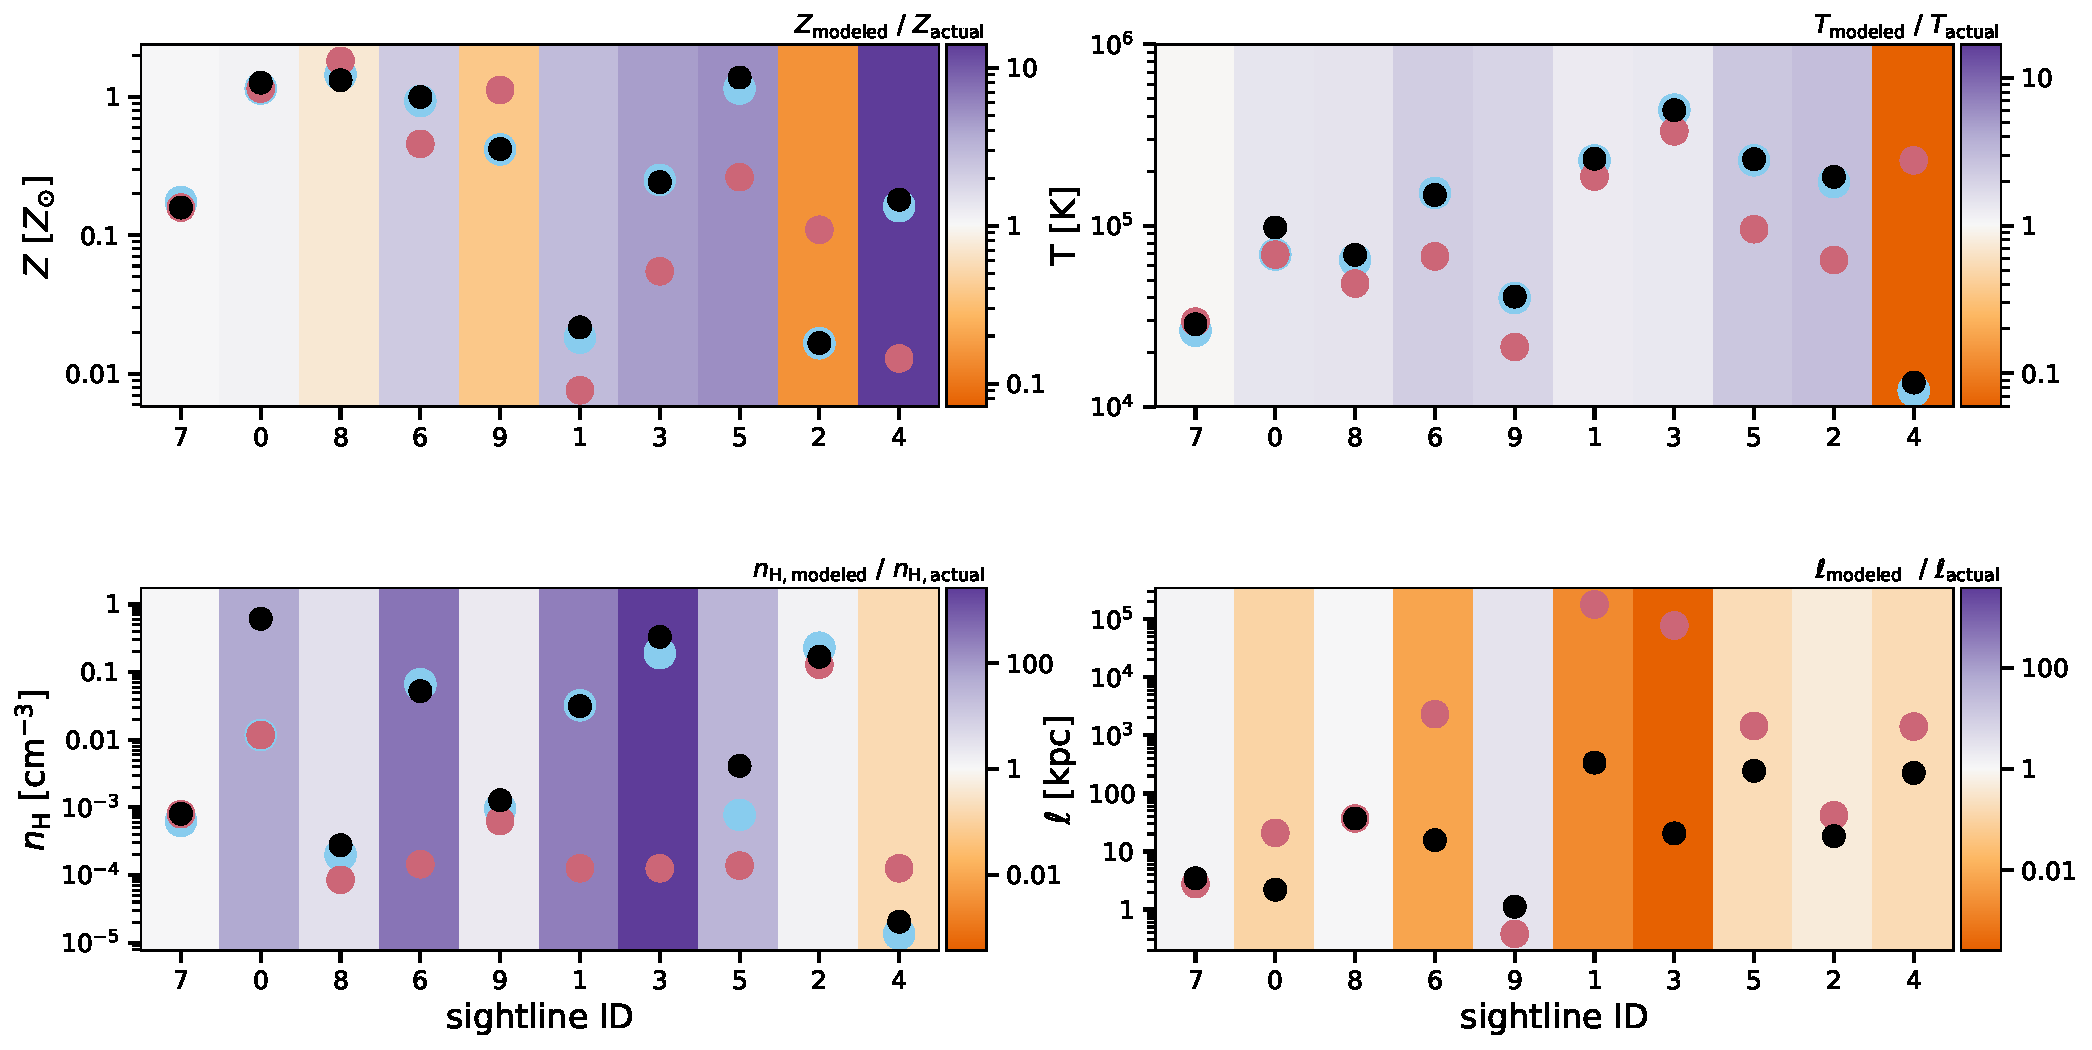
\includegraphics[width=\textwidth]{figures/sample0/comparison.pdf}
    \caption{
    Comparison in highly idealized scenario.
    }
    \label{f: idealized}
\end{figure*}

\begin{figure}
    \centering
    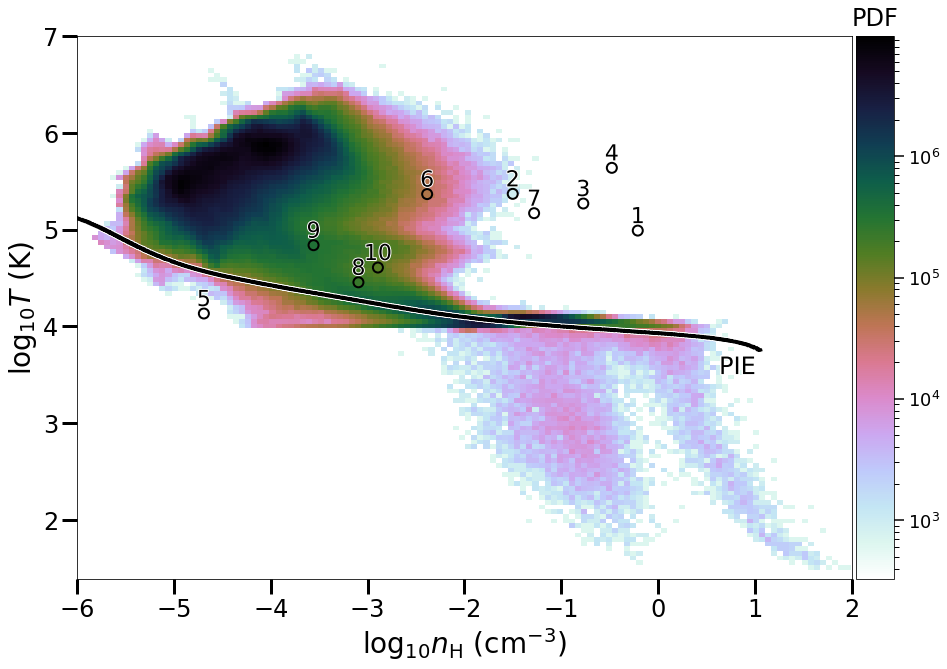
\includegraphics[width=\columnwidth]{figures/sample0/phase_space.png}
    \caption{
    \todo{Set colorbar by percent enclosed.}
    \todo{Use consistent axes: all log, or no log.}
    }
    \label{f: idealized explanation}
\end{figure}

\begin{figure*}
    \centering
    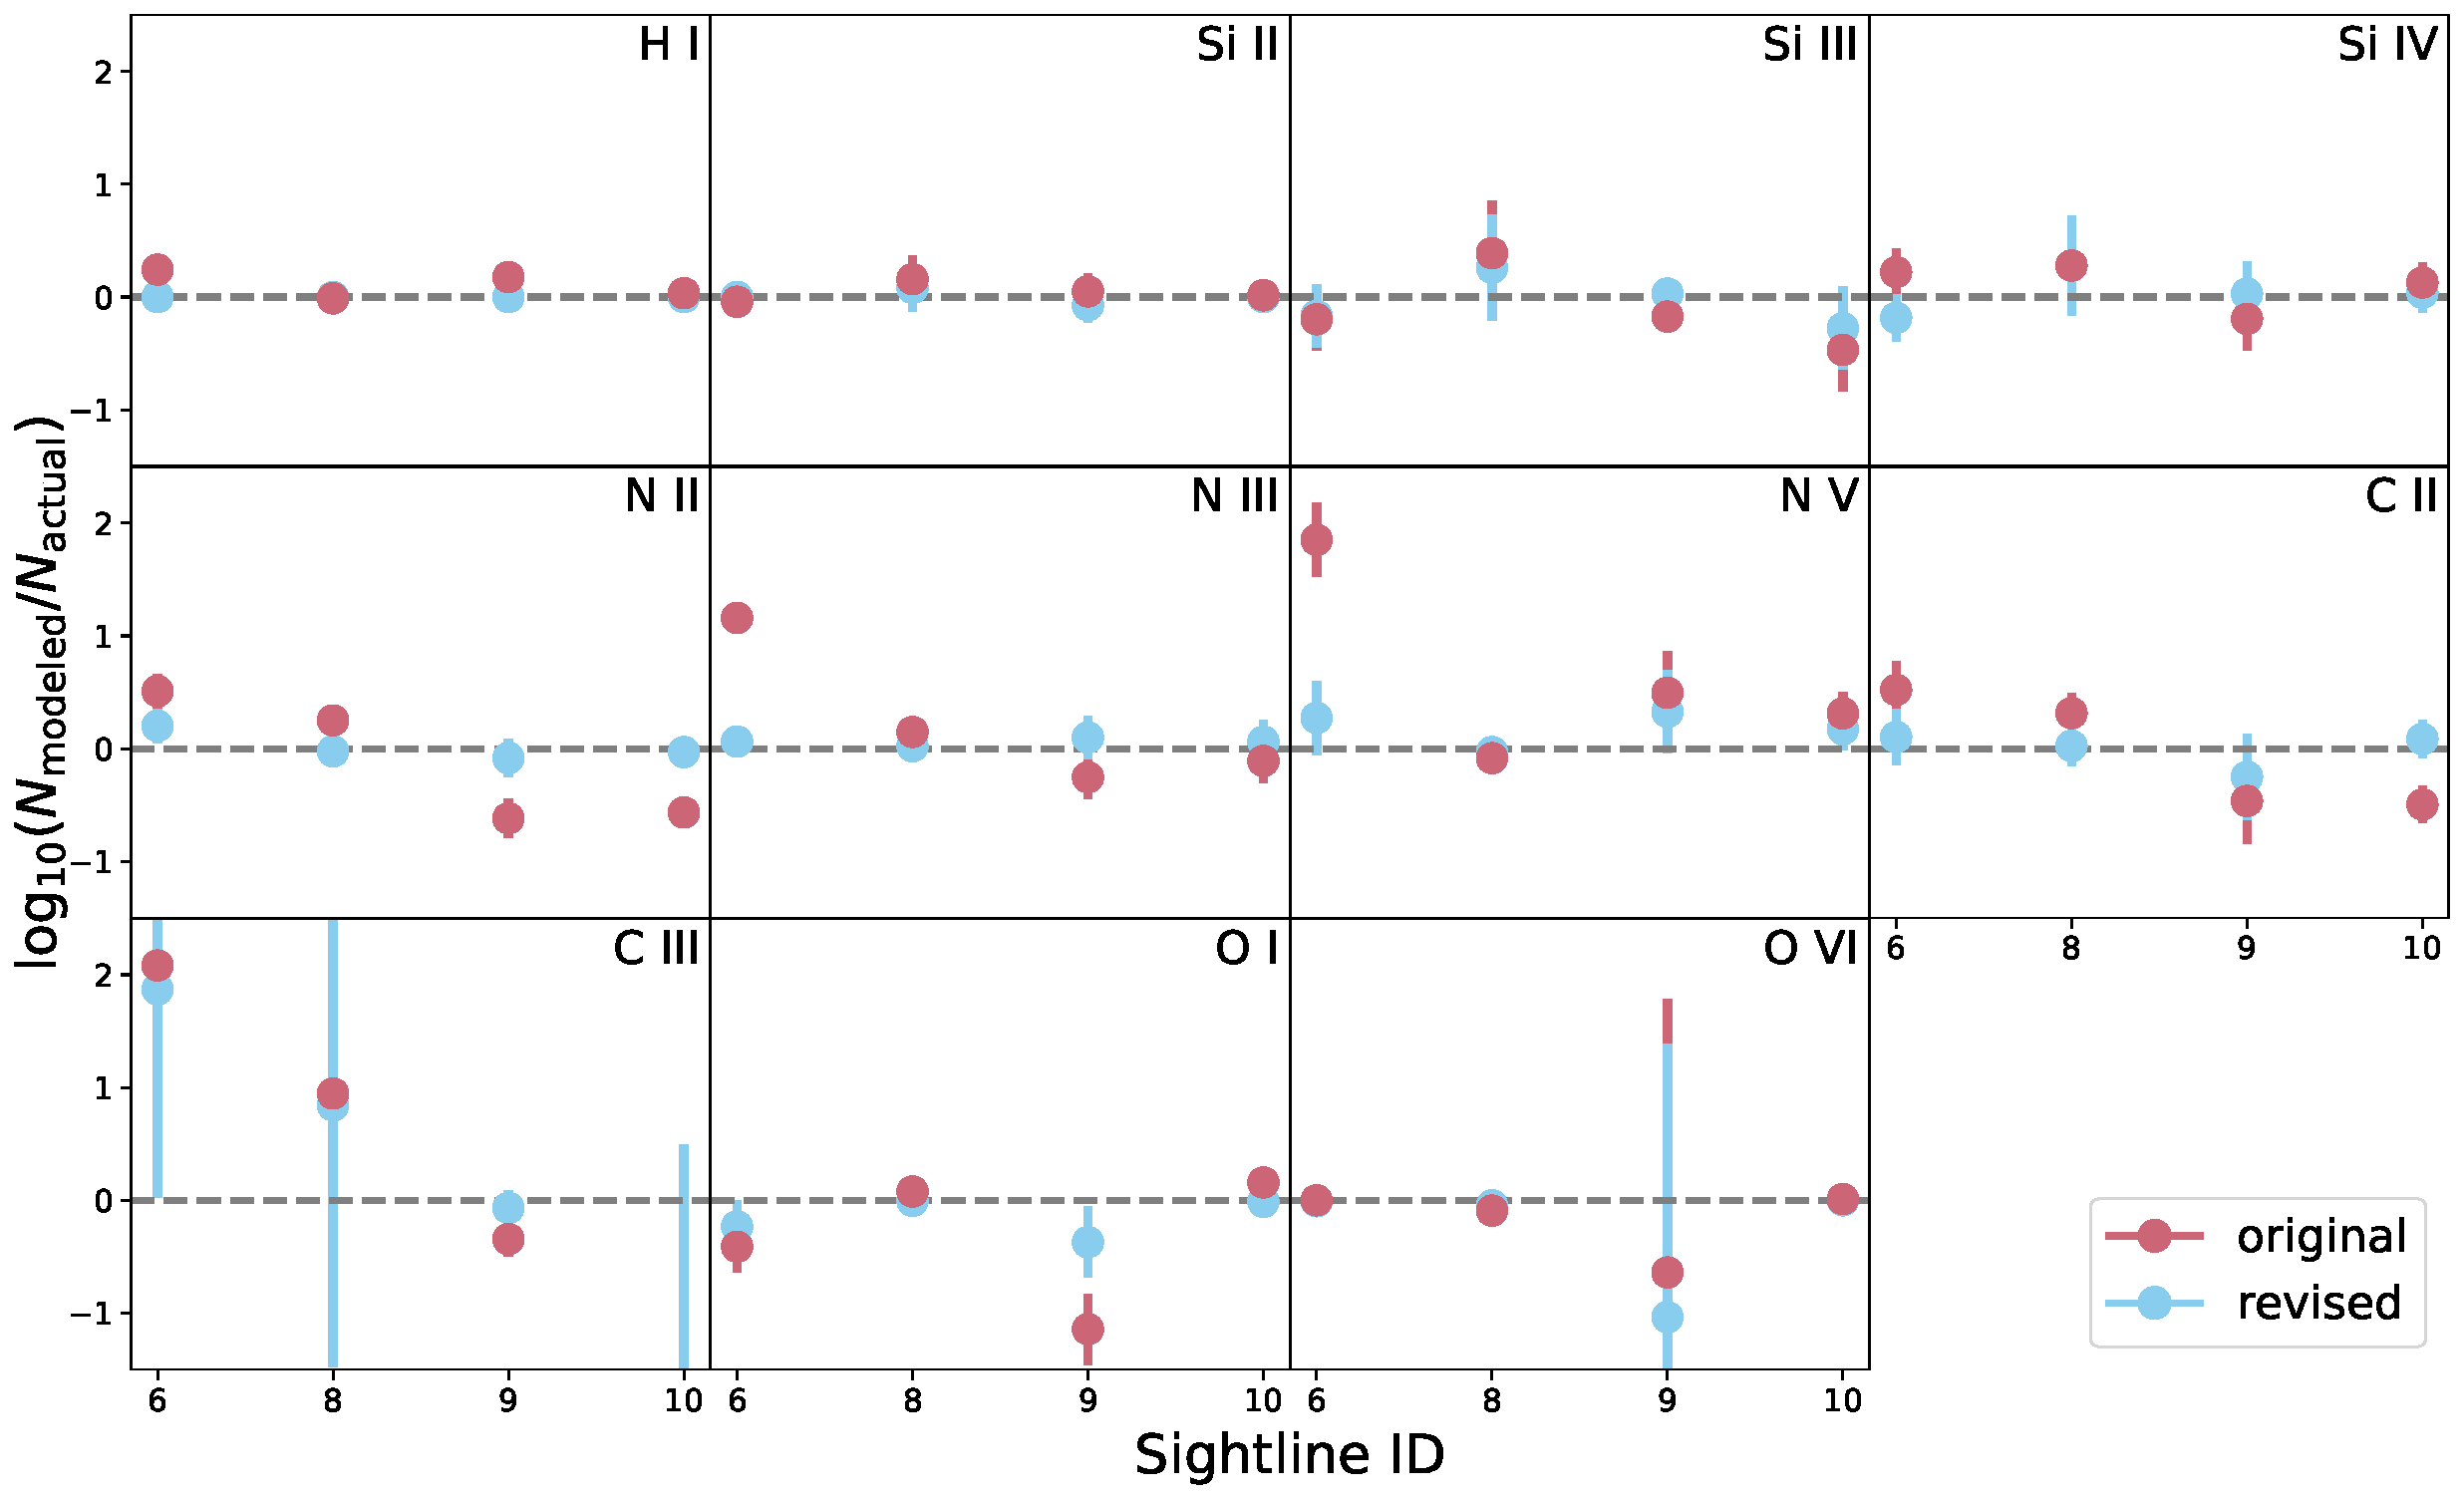
\includegraphics[width=\textwidth]{figures/sample0/column_den.pdf}
    \label{f: column density agreement}
\end{figure*}

% Results description
\todo{Add initial comparison figure description.}

% A tale of priors
The discrepancies between the modeled properties and the actual properties can be understood in the context of priors.
Data generators created \texttt{sample0} by randomly sampling properties from a uniform prior for each property, independent of other properties.
However, in combination the properties were often inconsistent with common expectations of CGM gas.
This is seen in Figure~\ref{f: idealized explanation}.
\todo{Add figure description.}
On the other hand, observers modeled \texttt{sample0} with priors constrained to regions of parameter space consistent with current knowledge of the CGM.
For example, observers tested if the column densities were consistent with photo-ionization equilibrium, in which case temperature depends on metallicity and density, and found reasonable fits for sightlines \texttt{06} through \texttt{10}.
Observers found reasonable fits for three of the other sightlines after fixing the density to $n_{\rm H} = 10^{-3.9}$ cm$^{-3}$ and assuming collisional ionization.
In the revised modeling observers used uniform priors, e.g. no ionization equilibrium assumptions, and found much better agreement with actual properties.
Even still, in four of the ten sightlines (\textsc{01}, \textsc{02}, \textsc{06}, \textsc{07}) the best fit parameters had total \ion{H} column densities unhandled by \textsc{cloudy}, which required observers to identify and scale solutions with the same ion densities but less total mass.

% Degenerate column densities
The above suggests reasonable agreement between modeled and actual ion column densities may be common, even when the modeled temperature, density, and metallicity are inconsistent with the actual values.
We explore this further in Figure~\ref{f: column density agreement}.
\todo{Add figure description.}
The properties of the revised models are in much better agreement with the actual properties, but the revised ion column densities are often within $\lesssim 0.5$ dex of the column densities first modeled.
A complicating element is that the errors data generators applied to the column densities were independent, e.g. $N_{\ion{H}{I},\,{\rm provided}} > N_{\ion{H}{I},{\rm ,actual}}$ does not mean $N_{\ion{Mg}{II},\,{\rm provided}} > N_{\ion{Mg}{II},\,{\rm actual}}$.

\atsameer{
Please feel free to add any additional commentary here, or to add in plots.
Anything I add in you're welcome to review, and I will do the same for you.
}

\atcameron{Given you generated the data, do you have additional thoughts?}

\subsection{Spectra of multi-cloud systems --- \texttt{sample1}}
\label{s: results -- sample1}

\begin{figure}
    \centering
    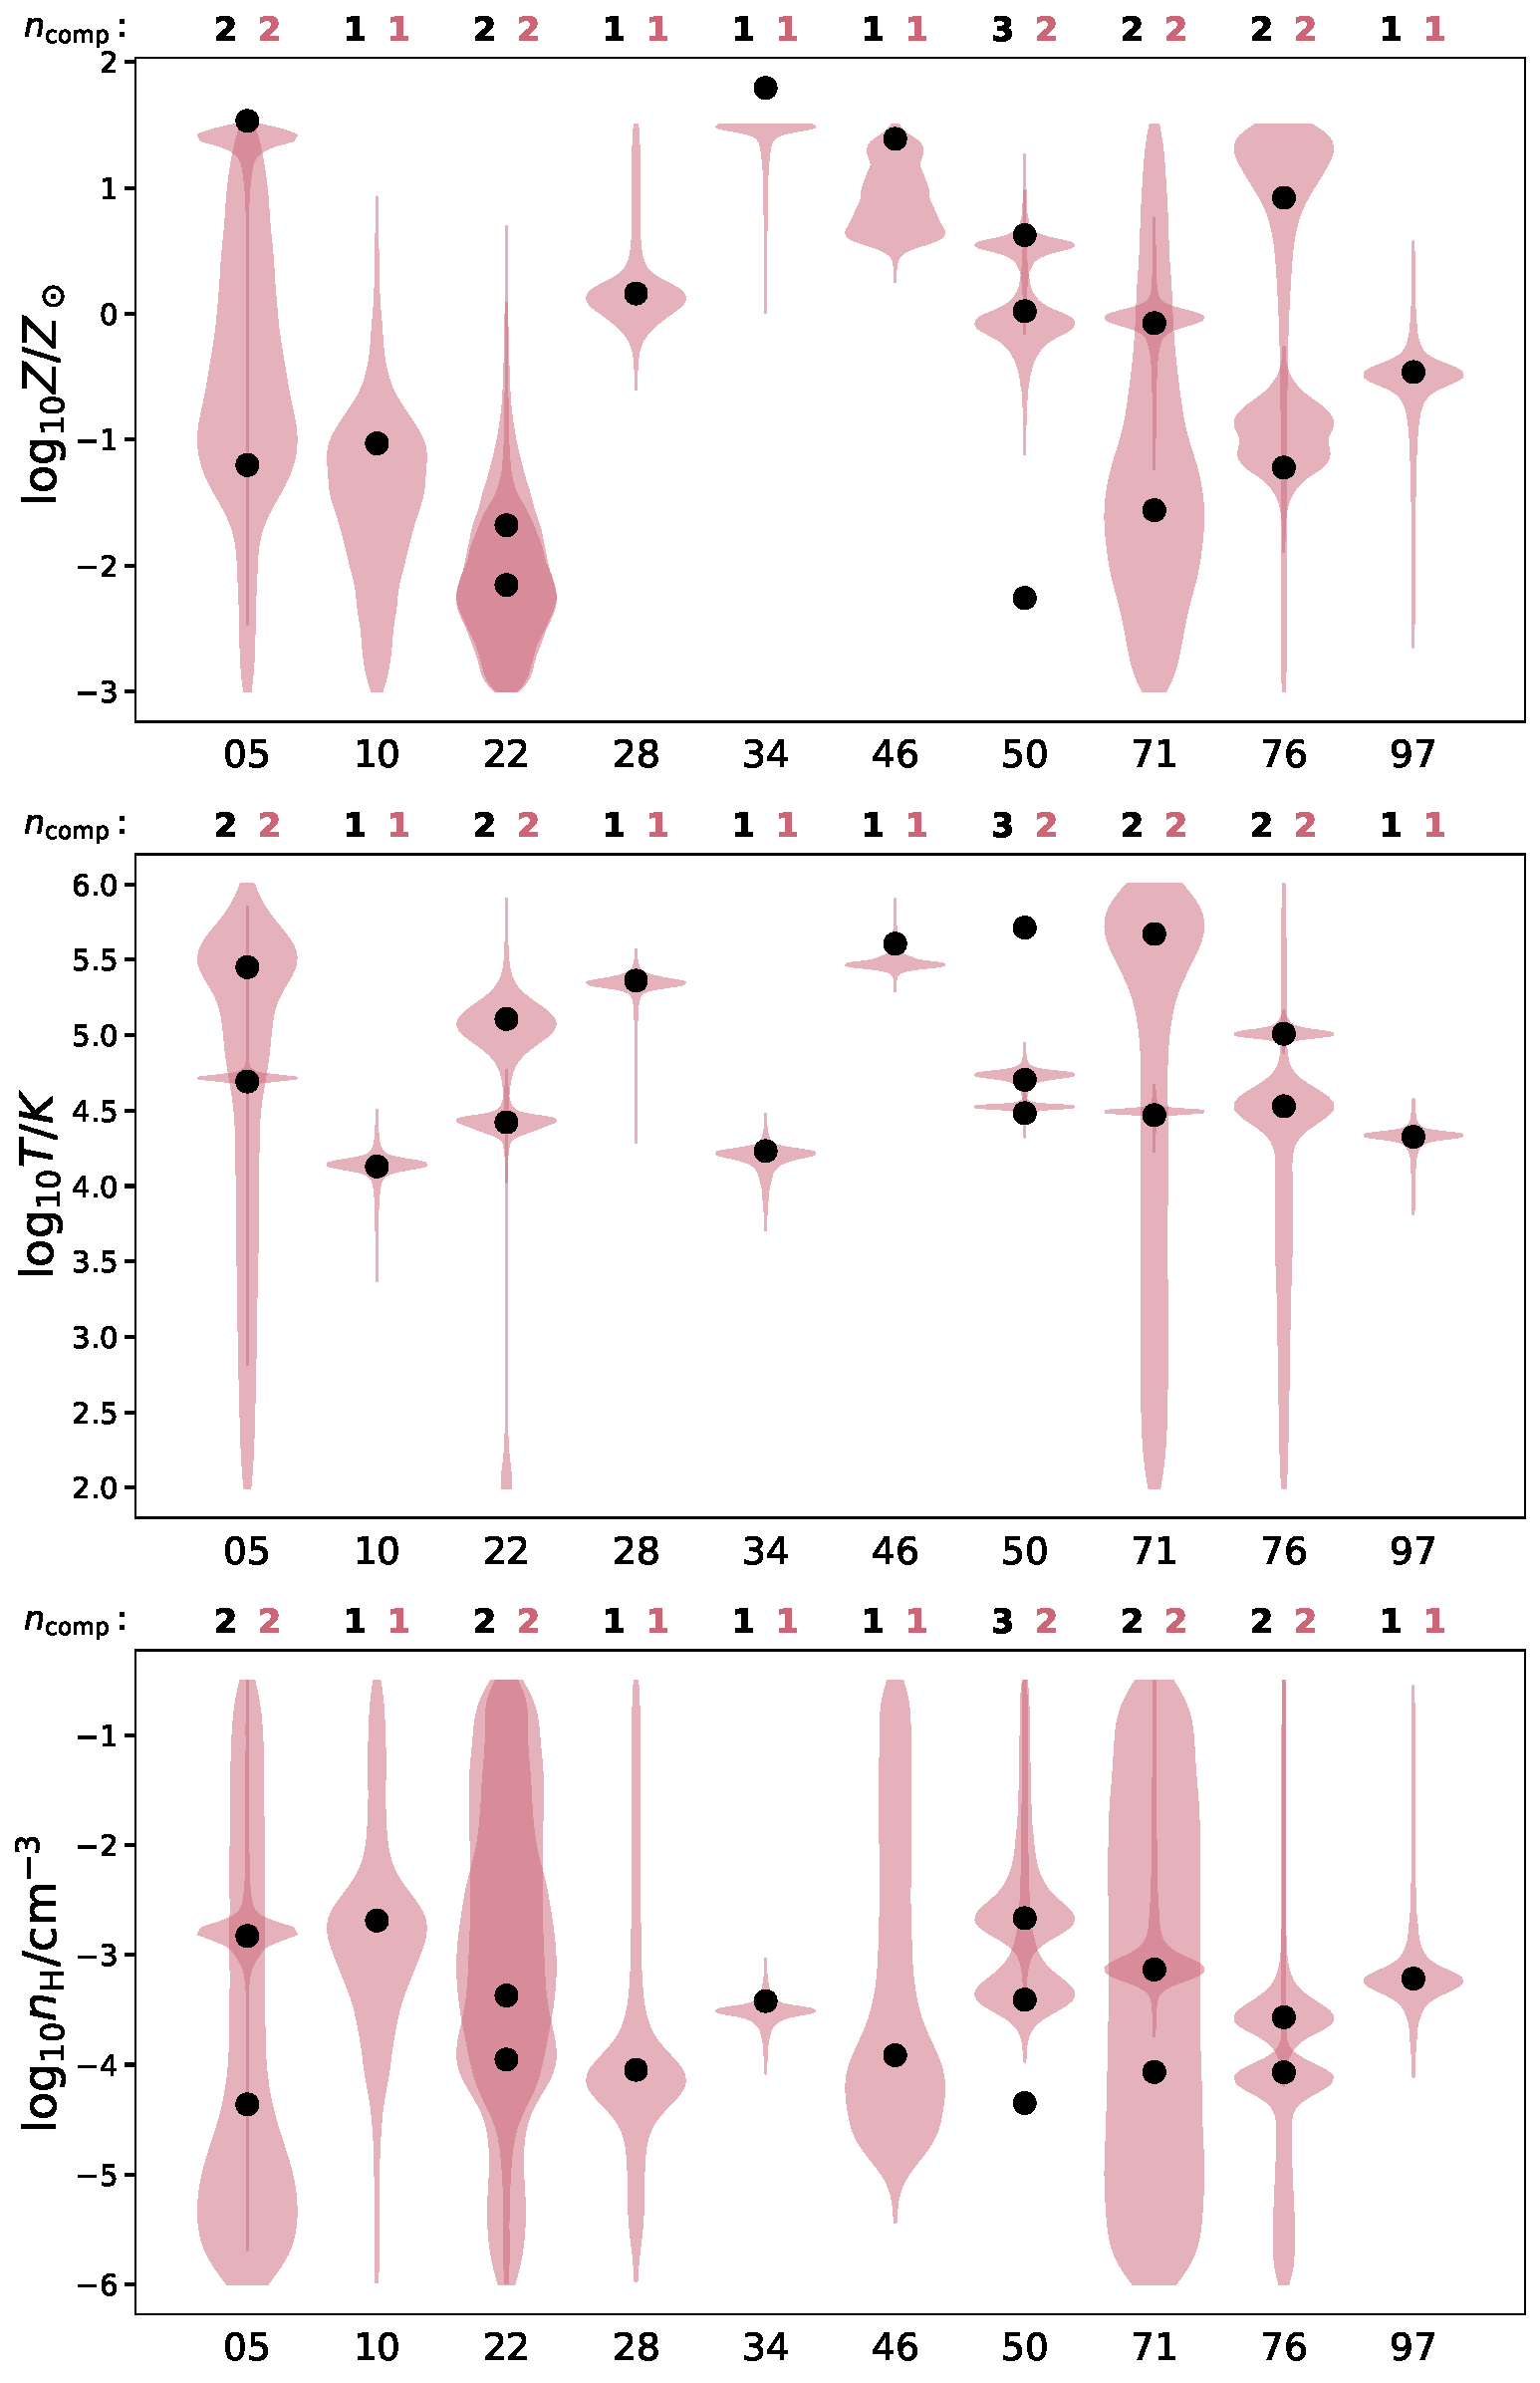
\includegraphics[width=\columnwidth]{figures/sample1/comparison.pdf}
    \caption{
    Comparison informed by cosmological simulations.
    }
    \label{f: informed}
\end{figure}

% Figure description
\todo{Add Figure~\ref{f: informed} description.}

% Width of posteriors and comparison to data
In most cases the actual value resides inside the modeled distributions of possible values, i.e. the posteriors.
In other words, the posteriors from modeling is, in most cases, sufficiently conservative.
The posteriors can span several dex, however the actual values often lie at the peak of the posteriors.
As with the blind modeling for \texttt{sample0} some actual values lie outside the priors used for modeling: some actual values have $Z > 10^{1.5} Z_\odot$, while the data was modeled with a uniform prior for $Z$ spanning $log_{10} Z/Z_\odot = [-3, 1.5]$.
However, the actual values are within $< 0.5$ dex of the upper edge of the posterior, significantly less discrepant than blind modeling for \texttt{sample0}.
\atsameer{Remind me why you limited the metallicity on the upper end?}
Typically temperature is well-constrained with the posterior often spanning $<0.1$ dex, while metallicity and density are more poorly constrained.
\atsameer{I recall you saying this is something you've also shown in recent work?}

% Number of components
The modeling identifies the correct number of components in 9 of 10 sightlines.
The exception is sightline 050, which has a hot, low-density, low-metallicity absorber that produces little absorption in the ions available for modeling.

\todo{Comparison of mass-weighted or \ion{H}{I}-weighted quantities.}

\atnastasha{Given your part in generating the data, do you have additional thoughts?}

\atsameer{Commentary for this sample?}

\subsection{Spectra of a high resolution simulation --- \texttt{sample2}}
\label{s: results -- sample2}

\begin{figure*}
    \centering
    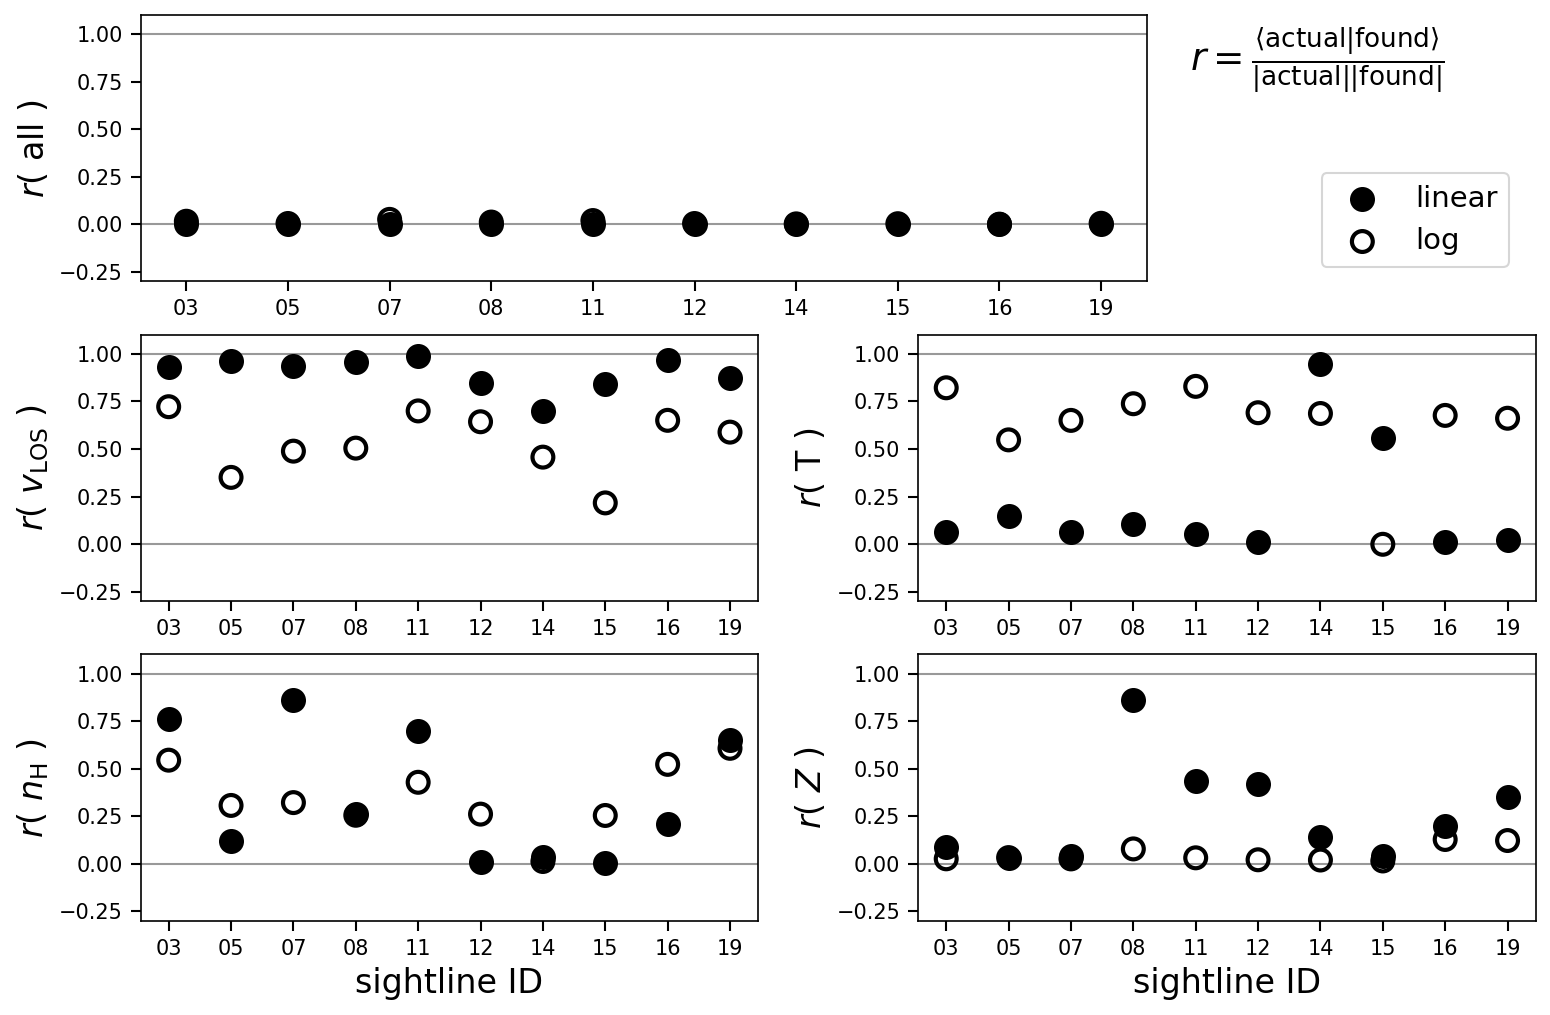
\includegraphics[width=\textwidth]{figures/sample2/correlations.png}
    \label{f: high-res}
    \caption{
    \todo{Use ``modeled'', not ``found''.}
    \todo{Cut out $r( {\rm all} )$.}
    }
\end{figure*}

\begin{figure*}
    \centering
    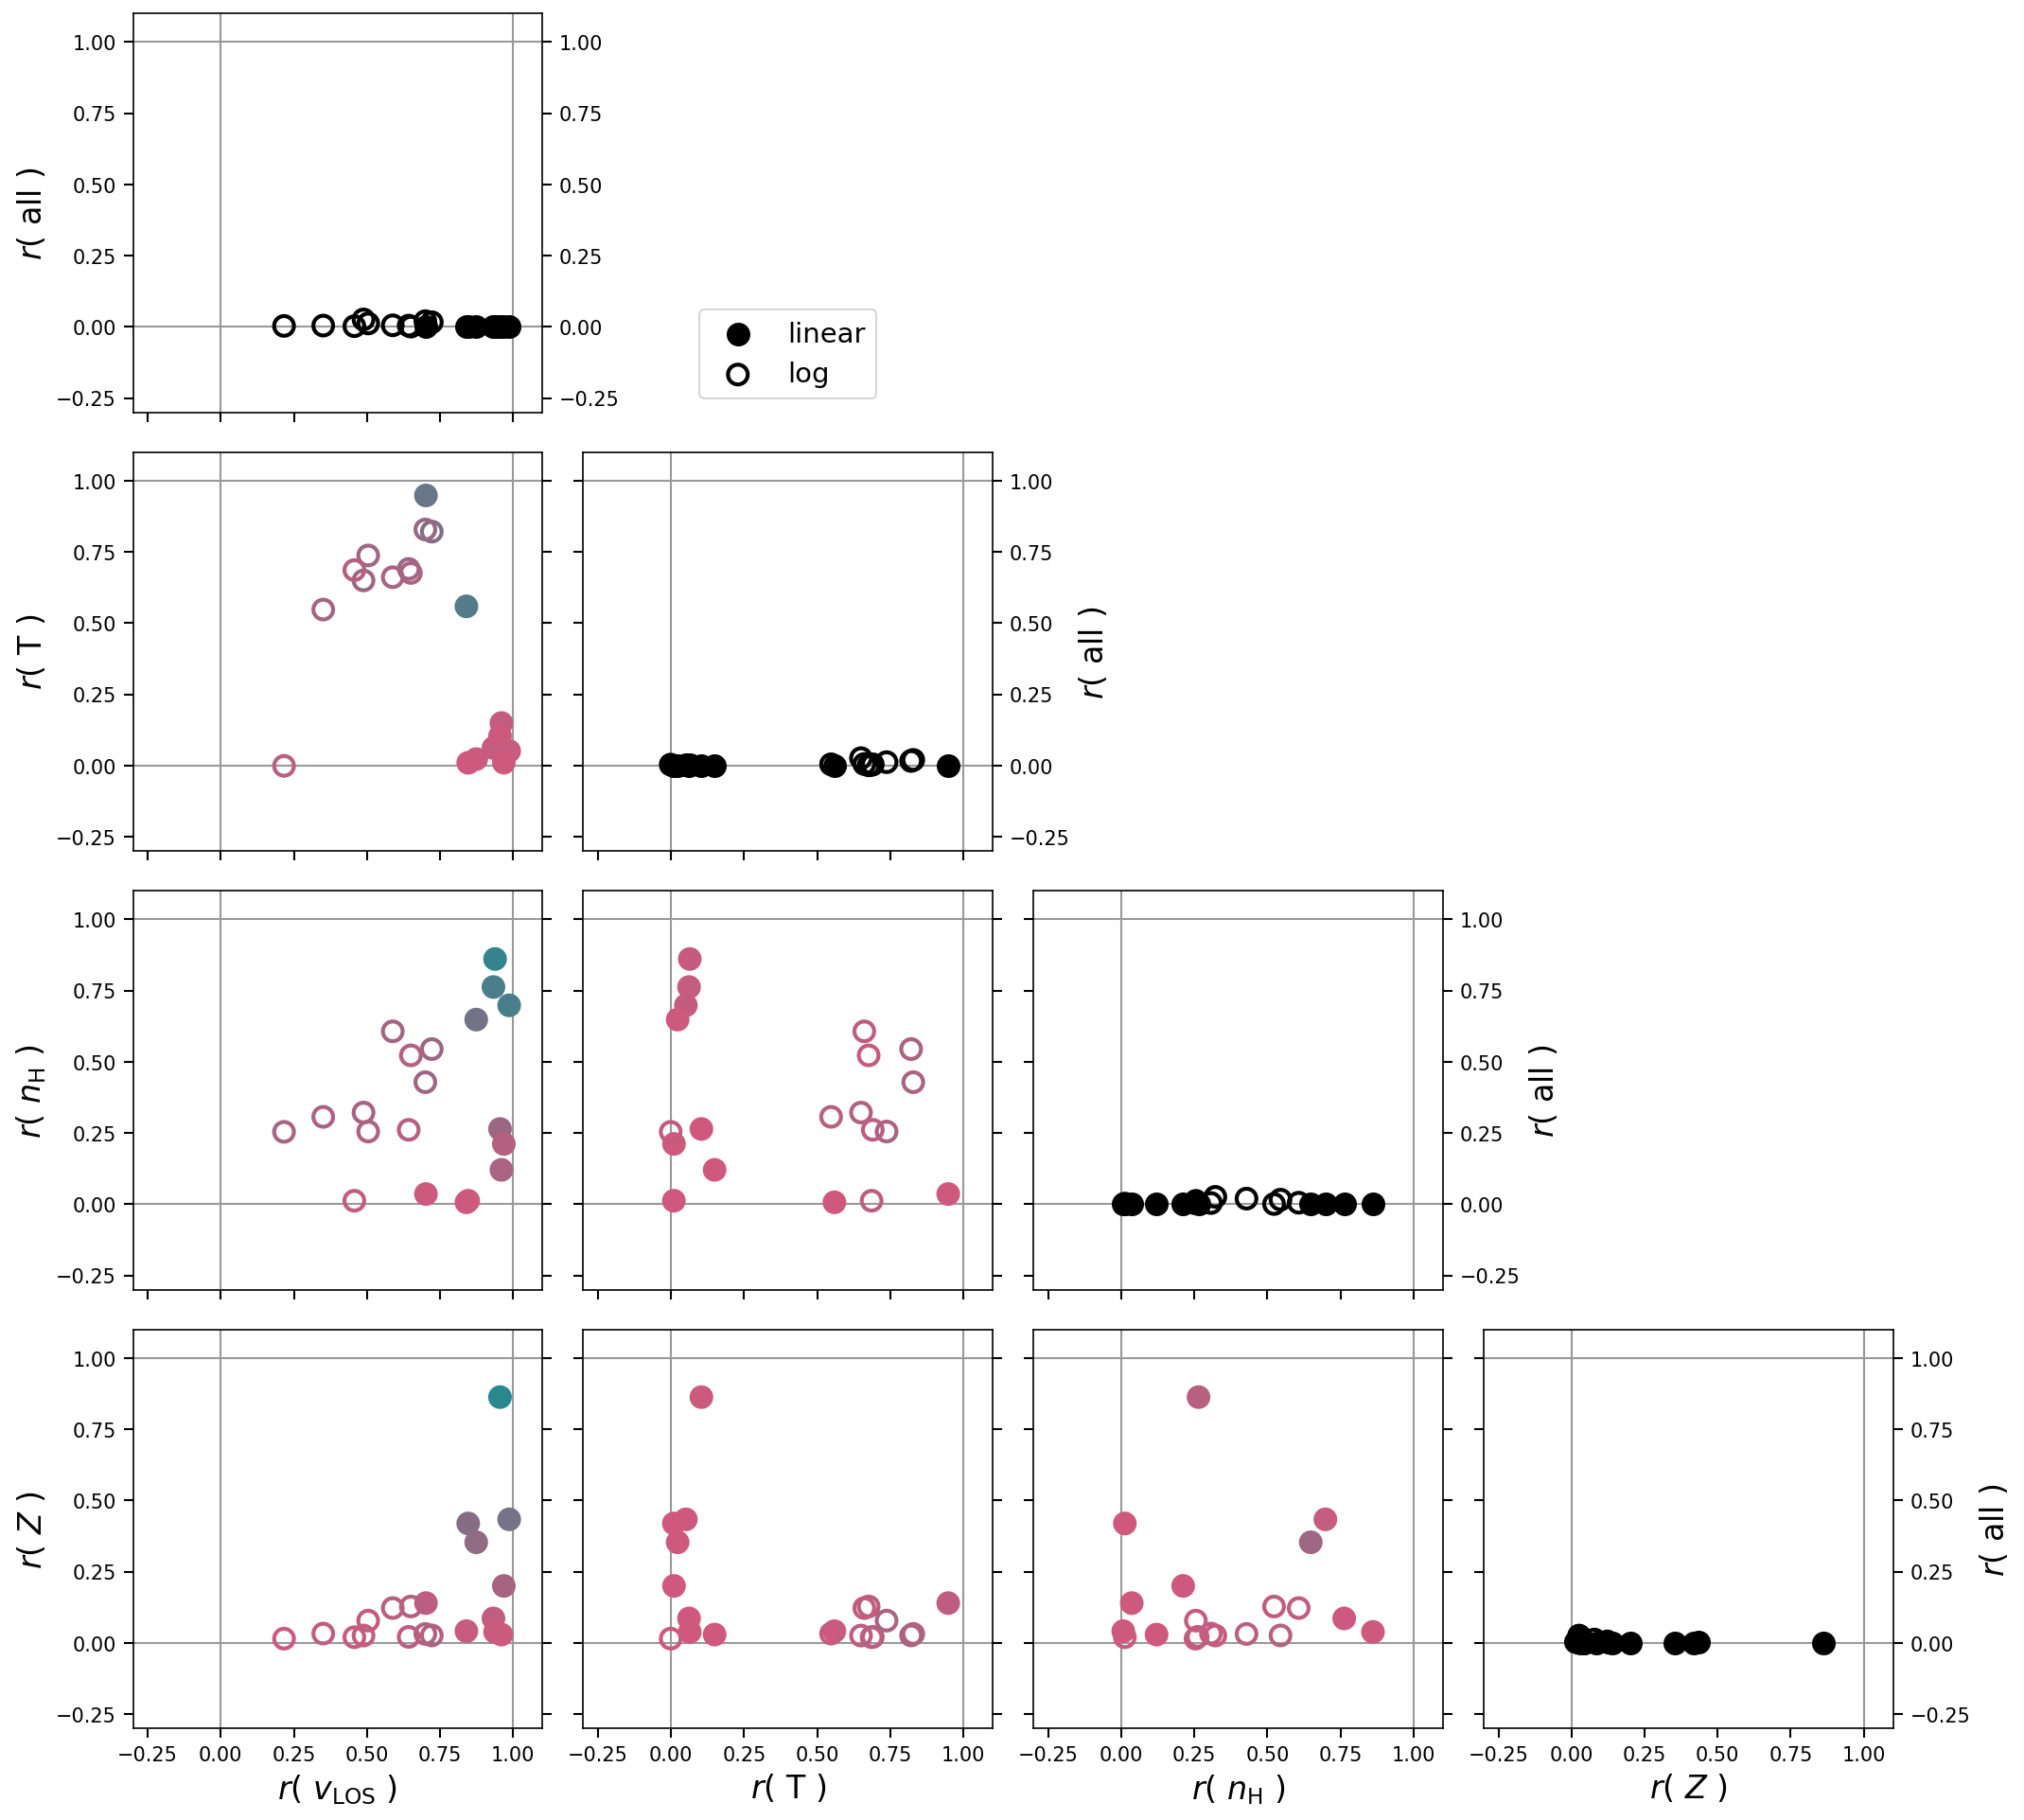
\includegraphics[width=\textwidth]{figures/sample2/correlations_corner.png}
    \label{f: high-res corner}
\end{figure*}

\begin{figure*}
    \centering
    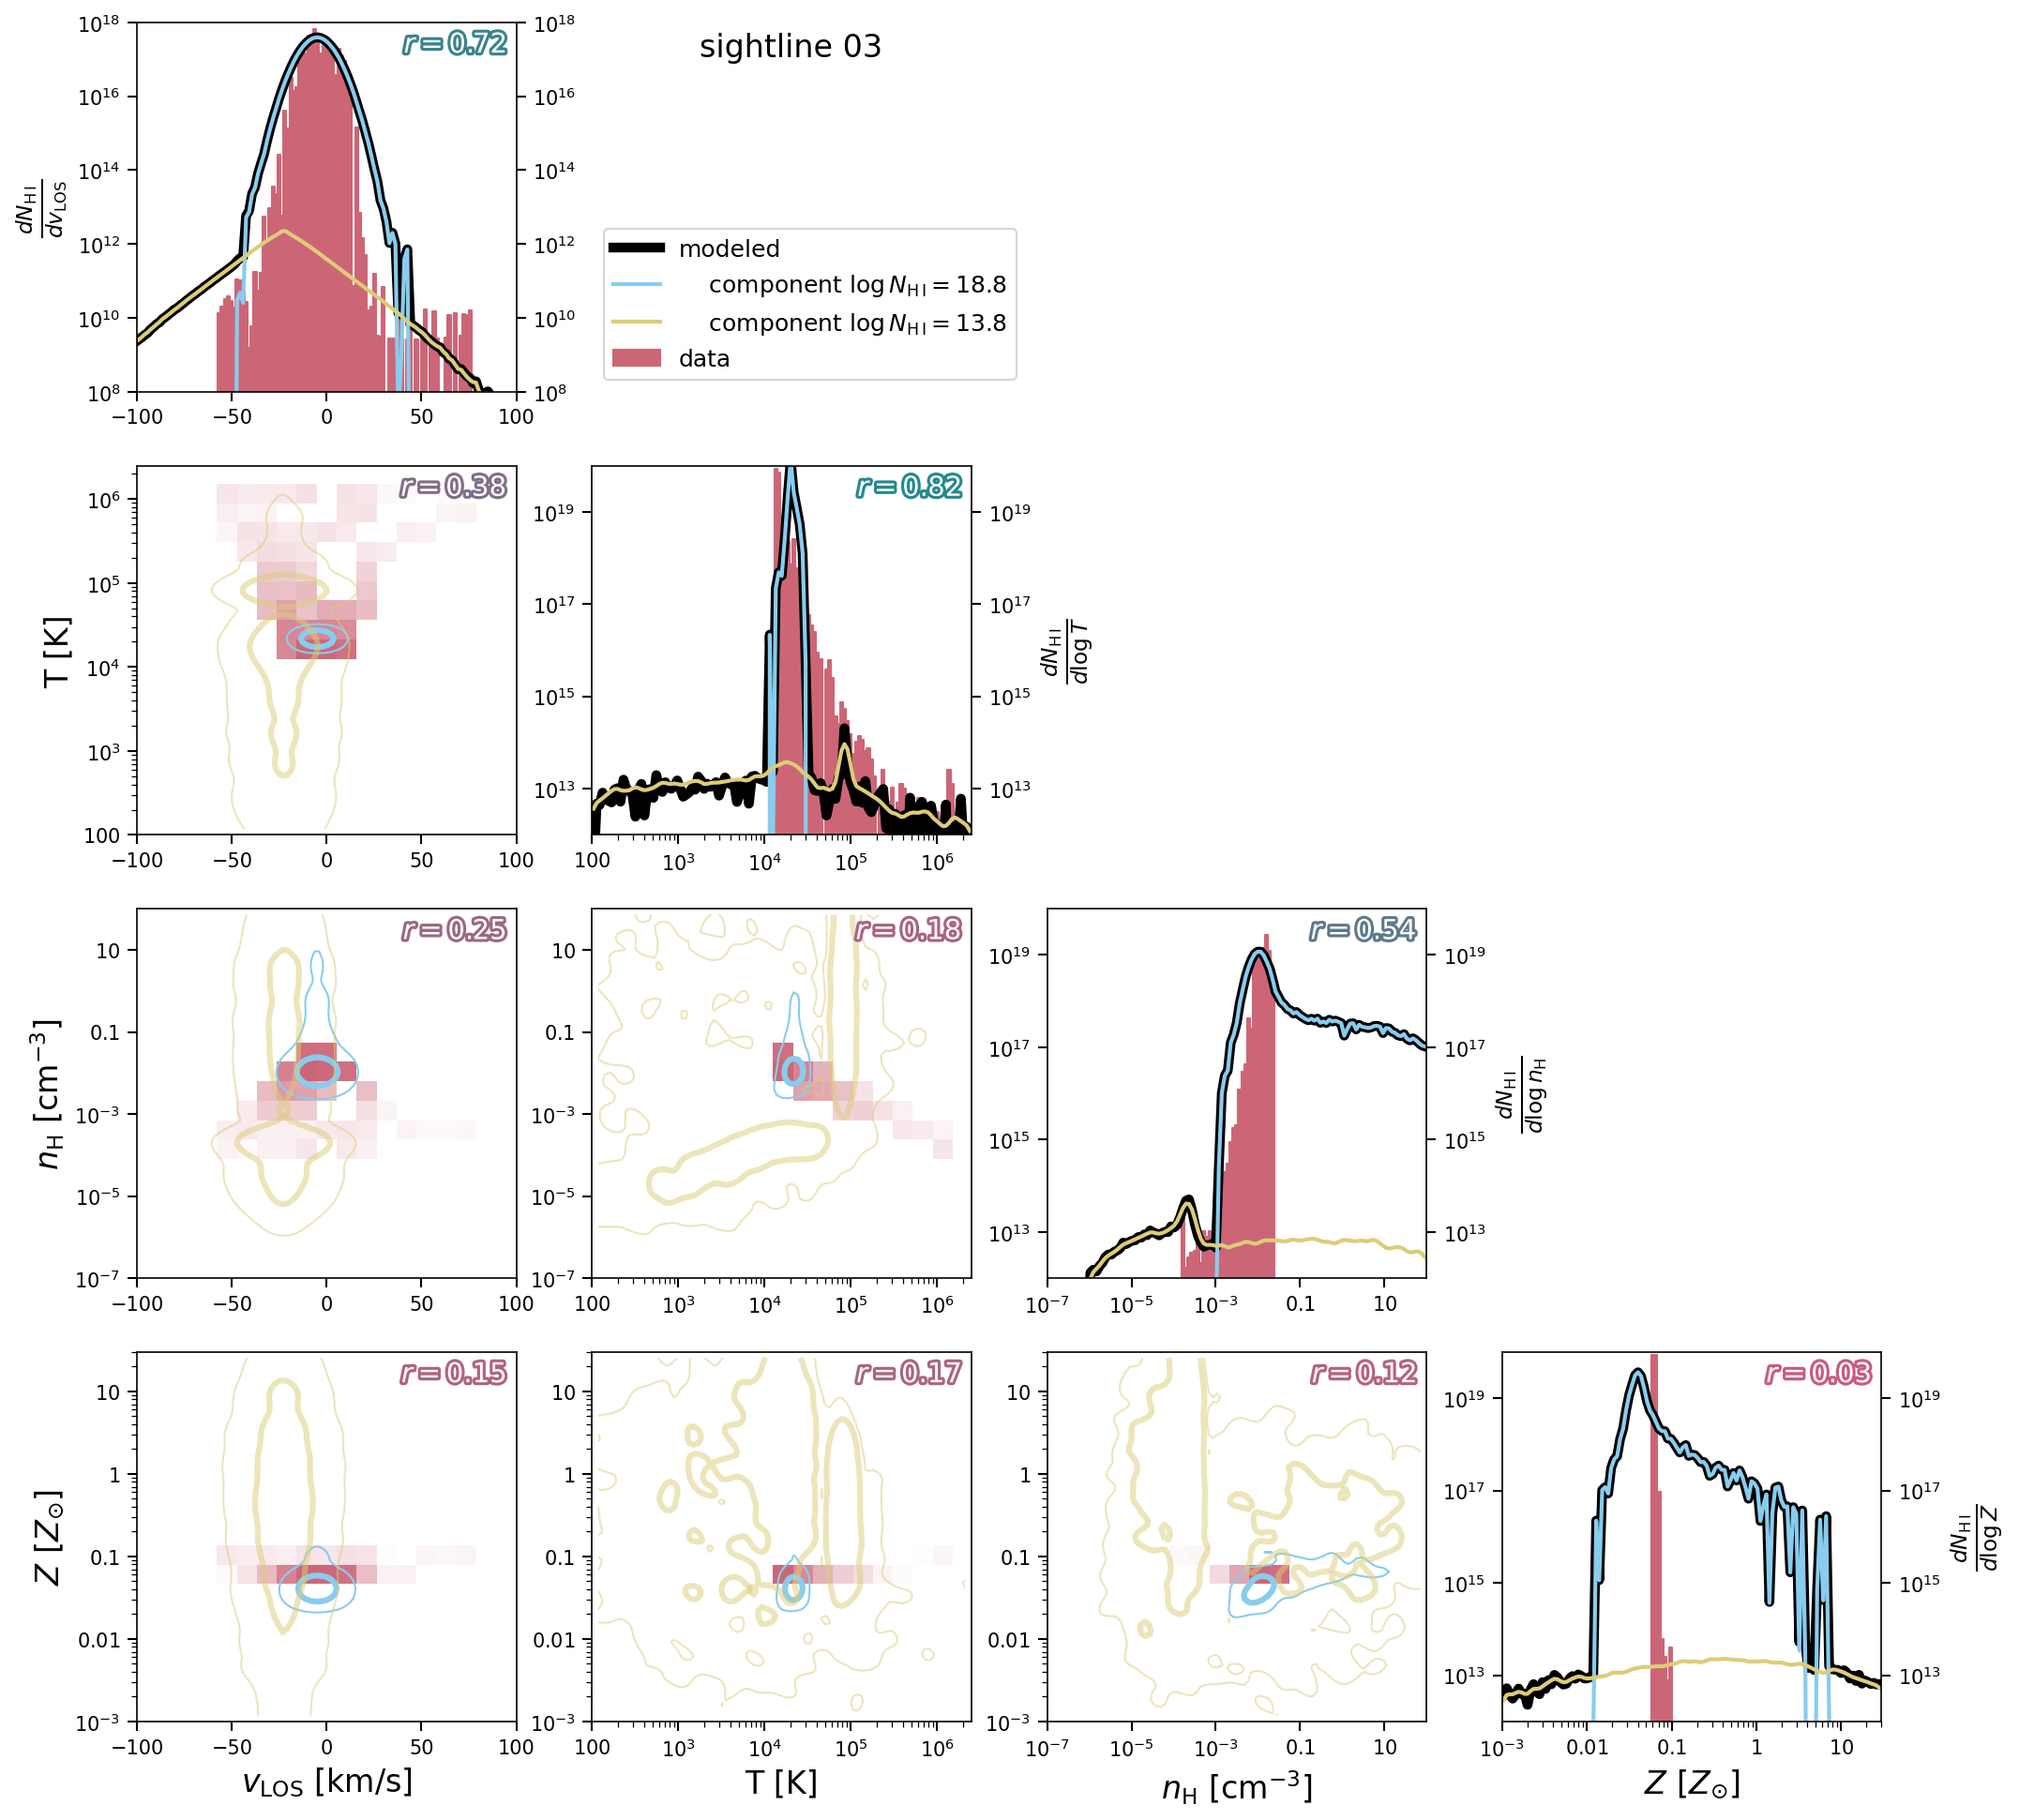
\includegraphics[width=\textwidth]{figures/sample2/sightline_0003.png}
    \label{f: sample2 03}
\end{figure*}

\begin{figure*}
    \centering
    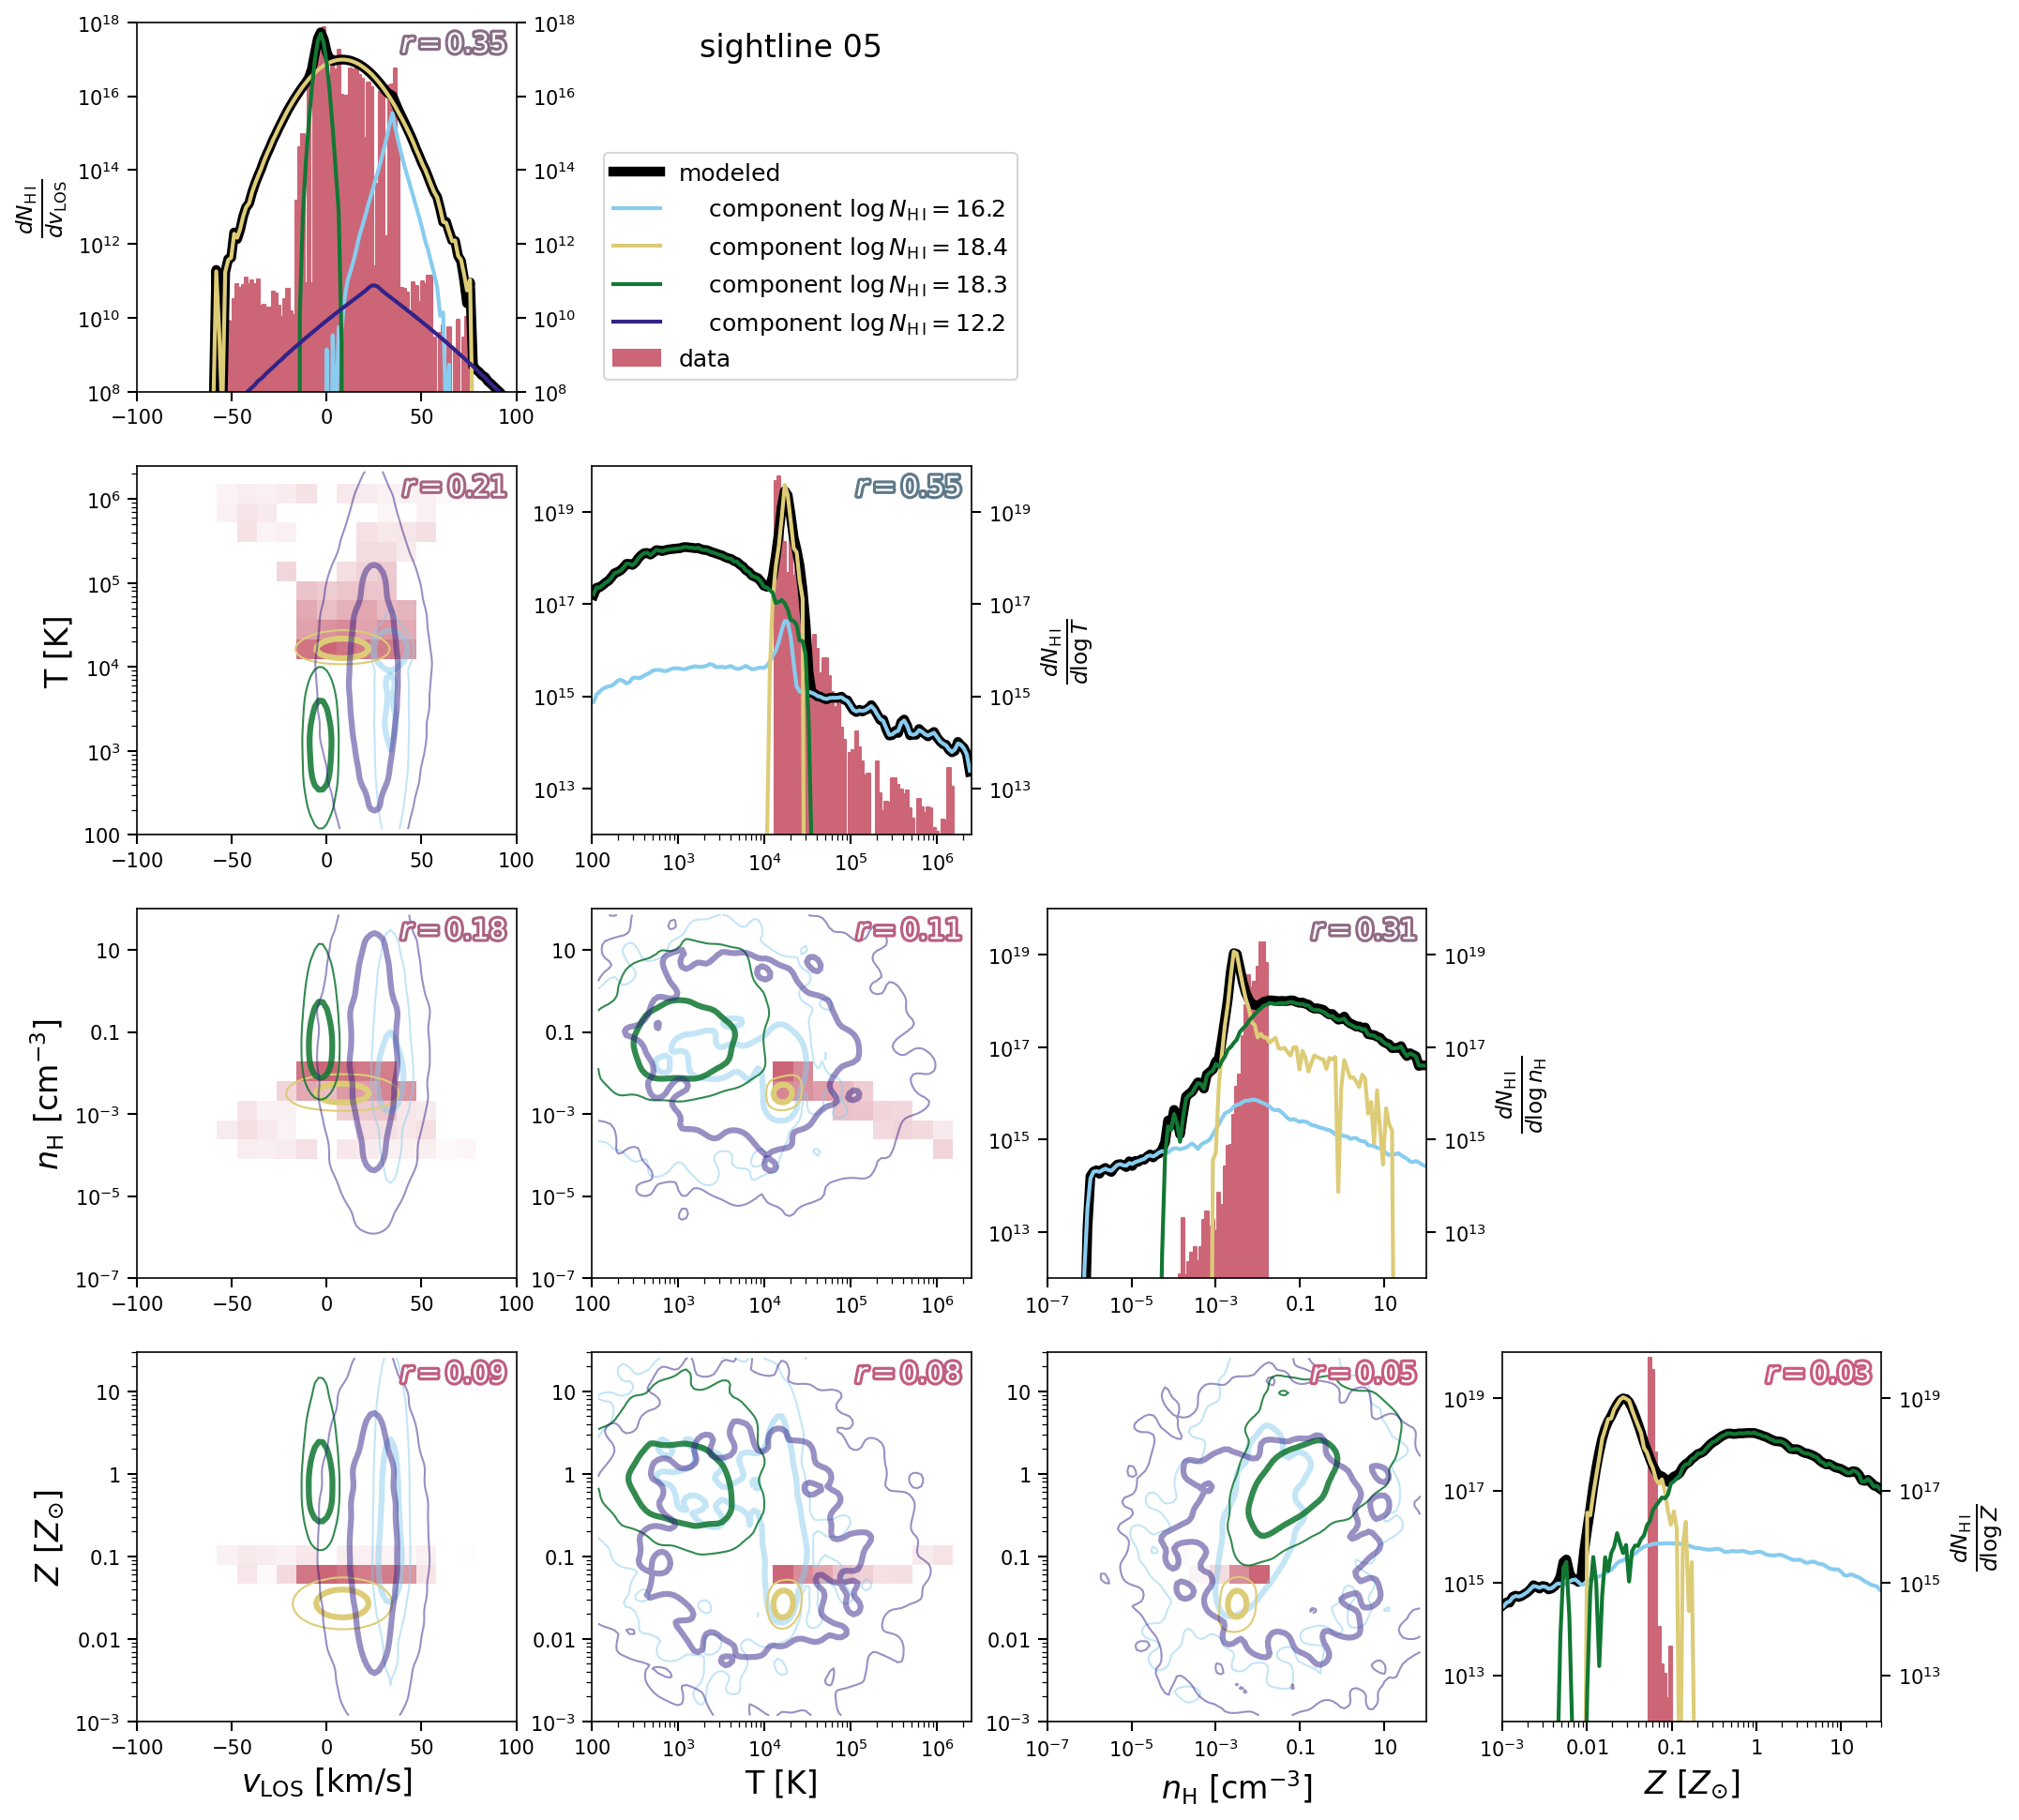
\includegraphics[width=\textwidth]{figures/sample2/sightline_0005.png}
    \label{f: sample2 05}
    \caption{Same as Fig.~\ref{f: sample2 03}, but for sightline 05.}
\end{figure*}

\begin{figure*}
    \centering
    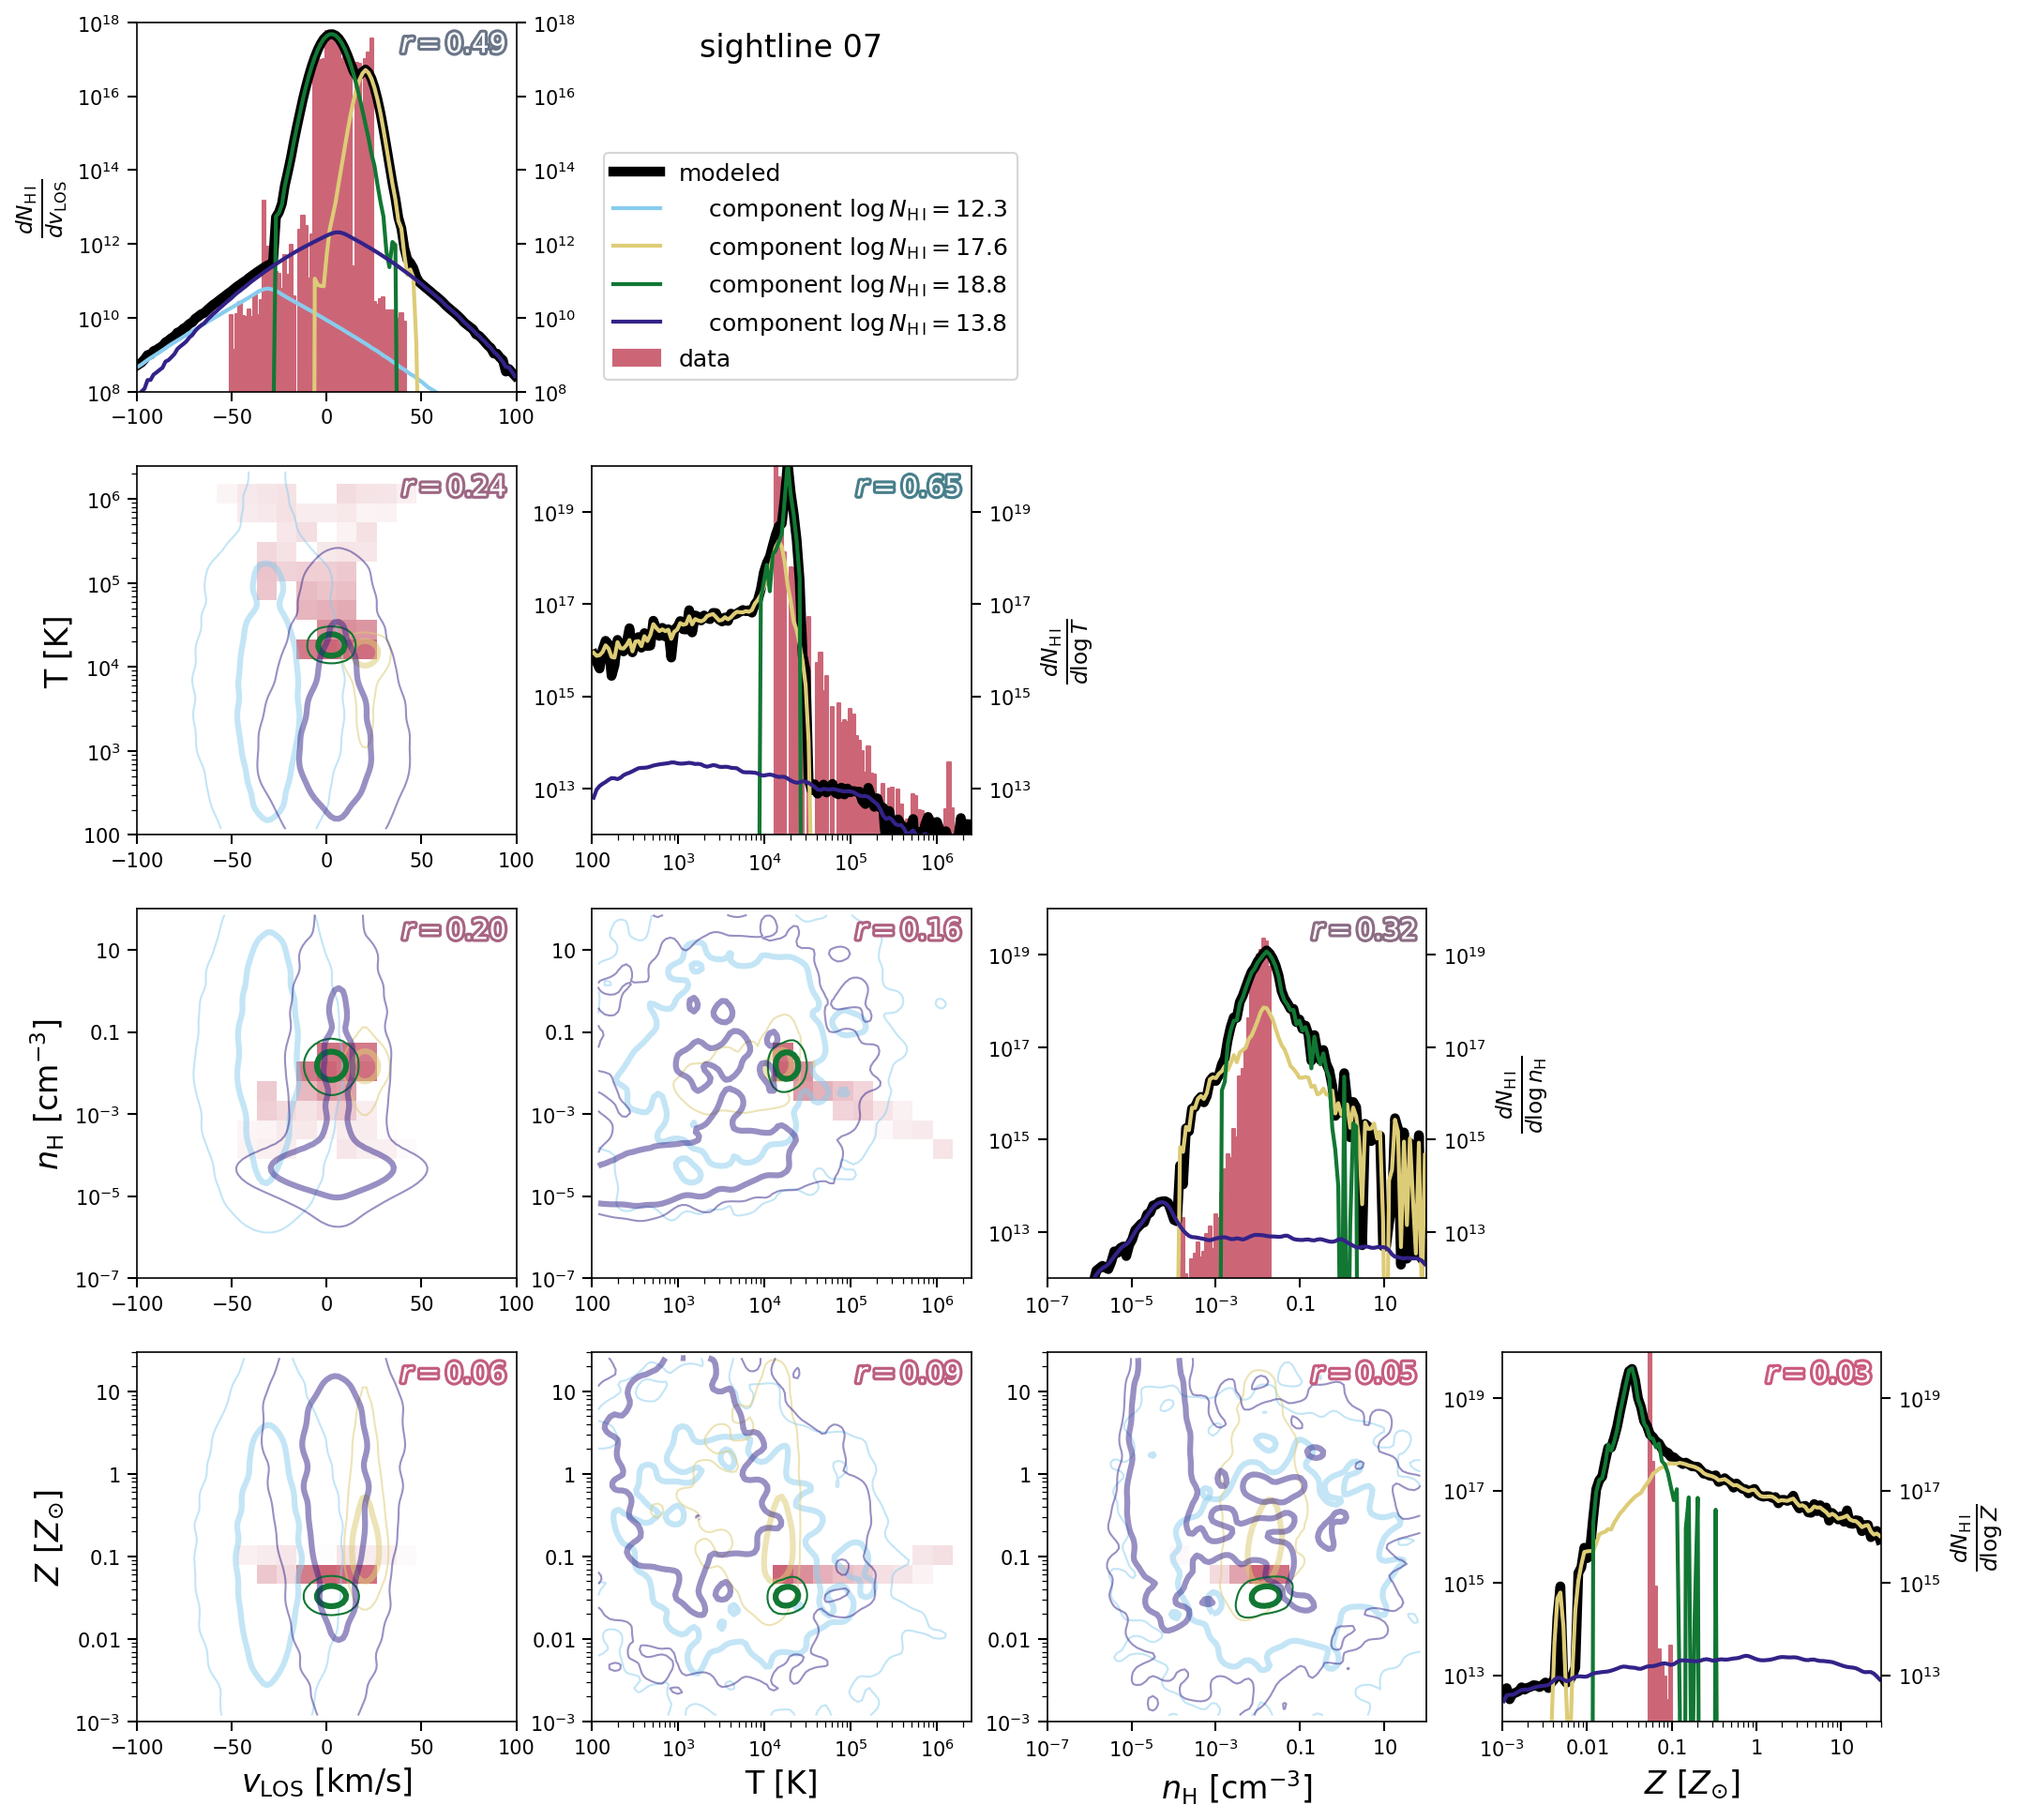
\includegraphics[width=\textwidth]{figures/sample2/sightline_0007.png}
    \label{f: sample2 07}
    \caption{Same as Fig.~\ref{f: sample2 03}, but for sightline 07.}
\end{figure*}

\begin{figure*}
    \centering
    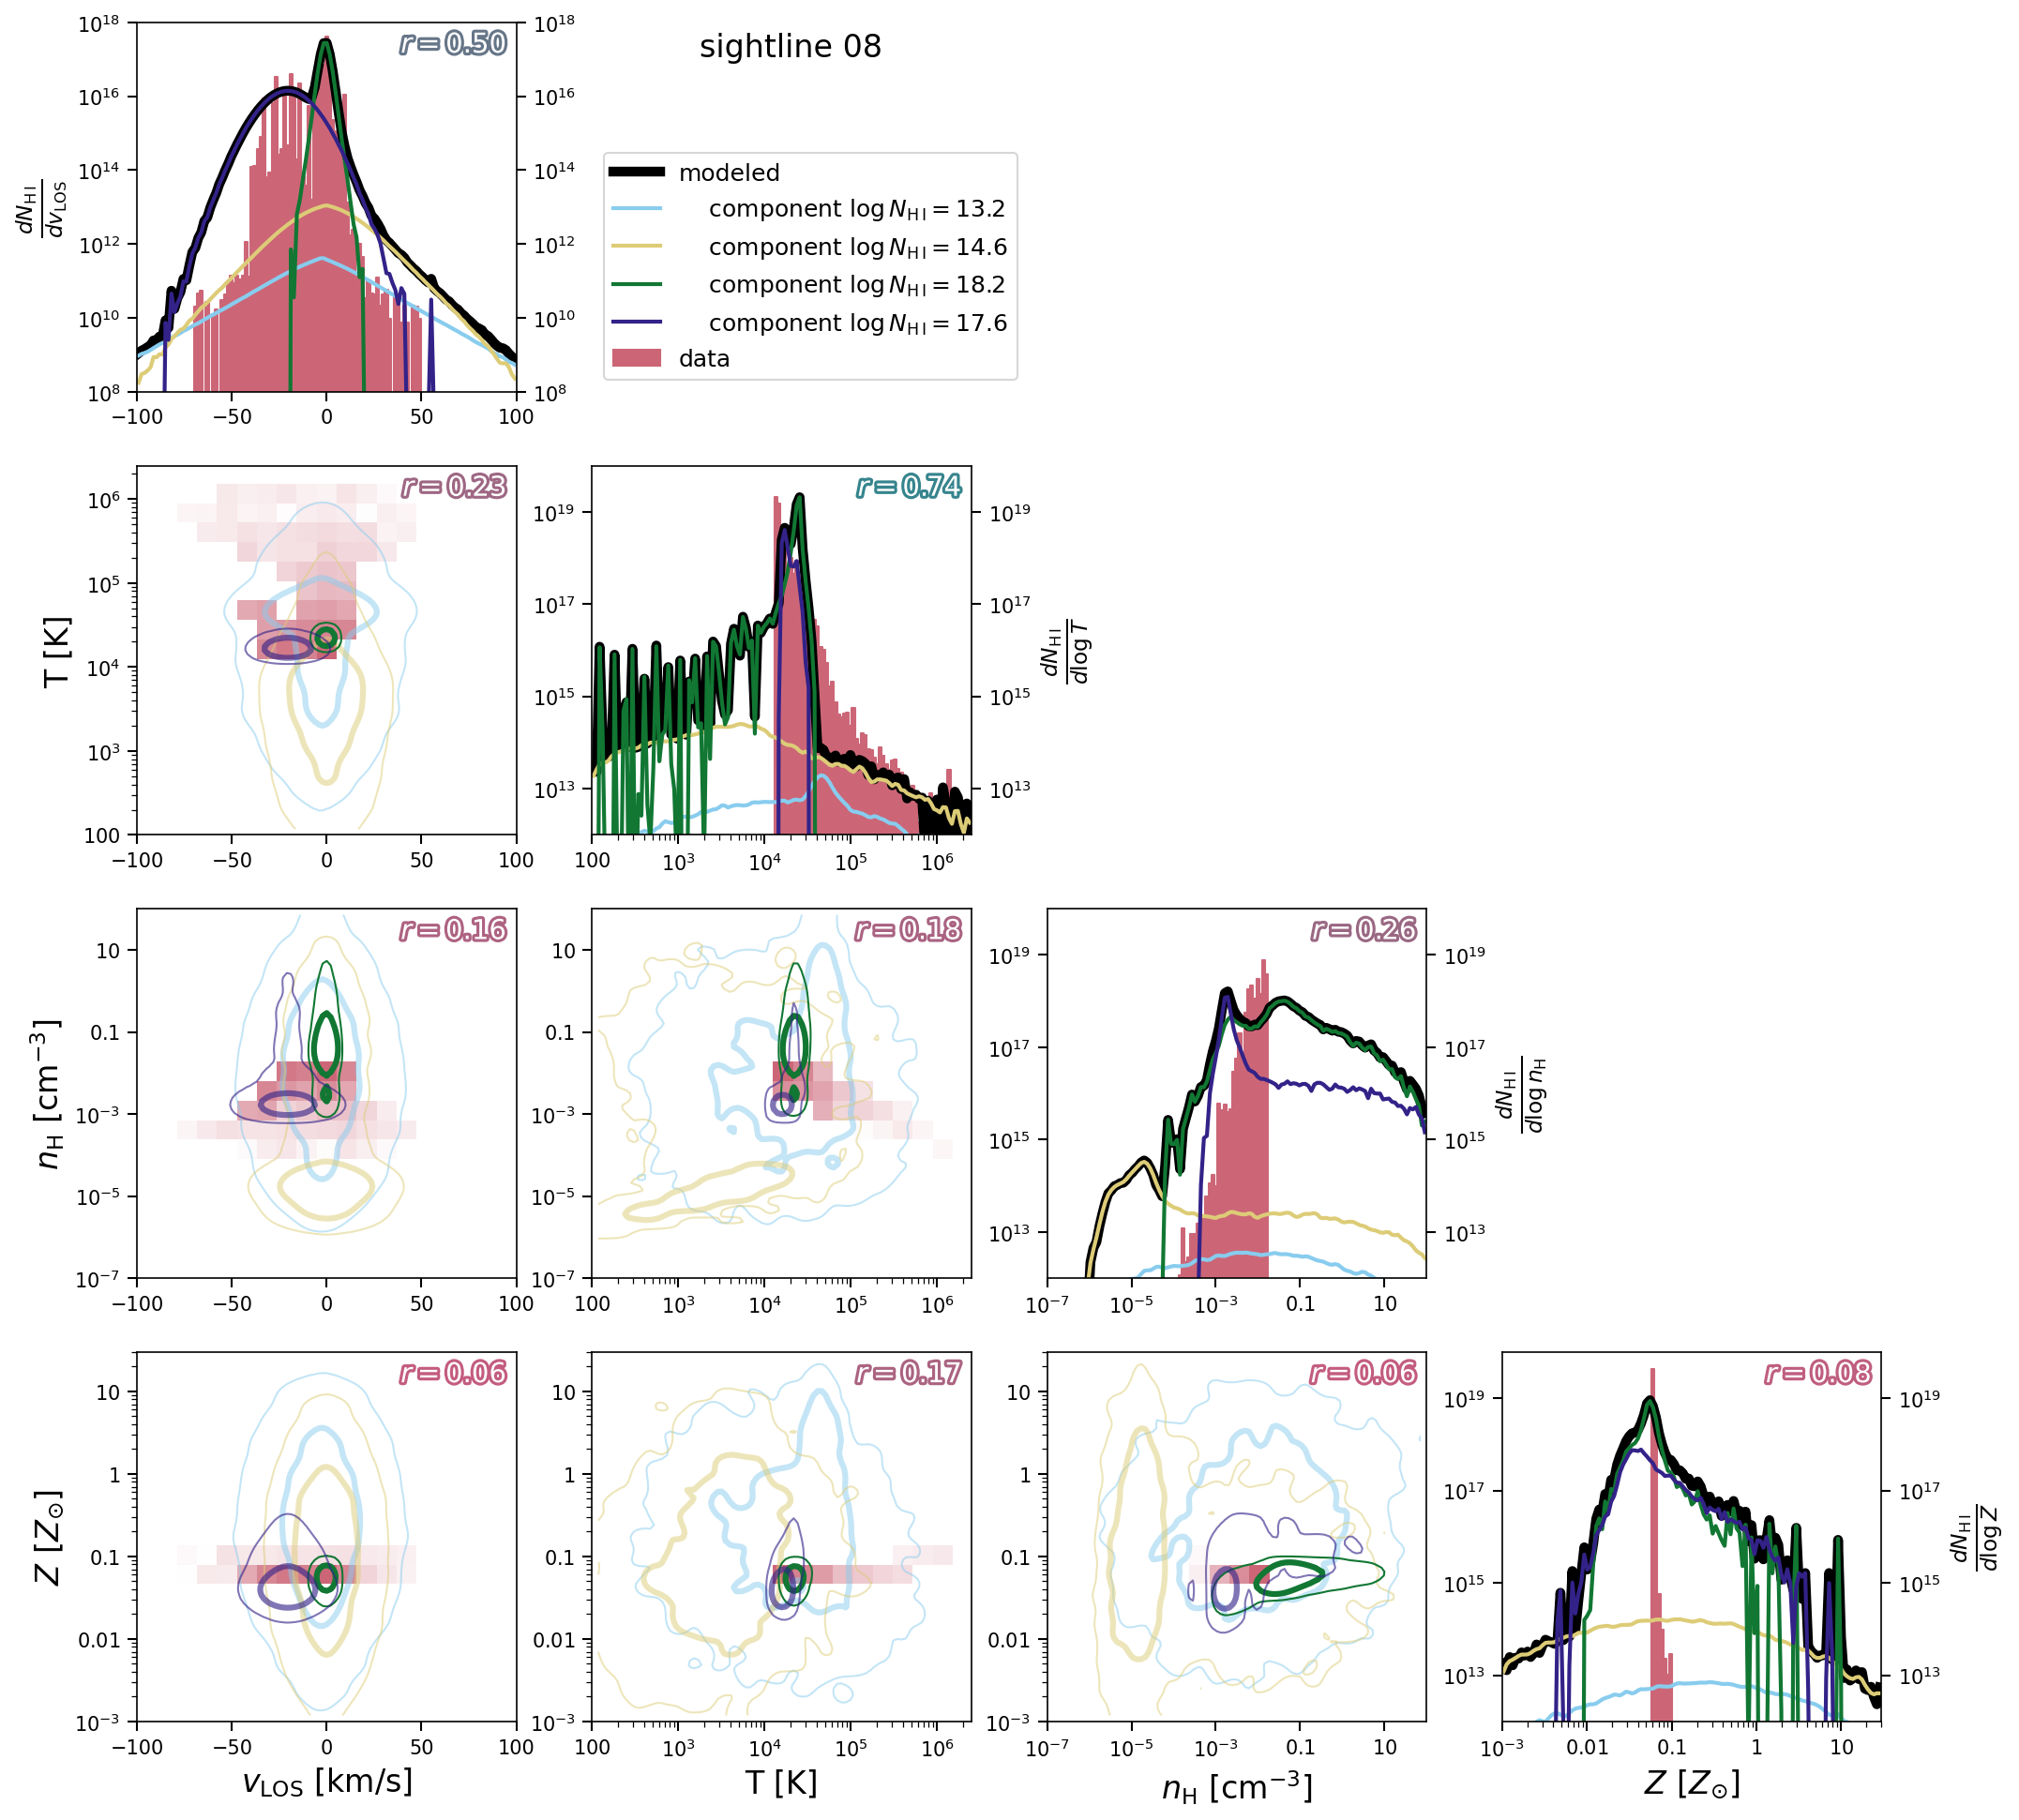
\includegraphics[width=\textwidth]{figures/sample2/sightline_0008.png}
    \label{f: sample2 08}
    \caption{Same as Fig.~\ref{f: sample2 03}, but for sightline 08.}
\end{figure*}

\begin{figure*}
    \centering
    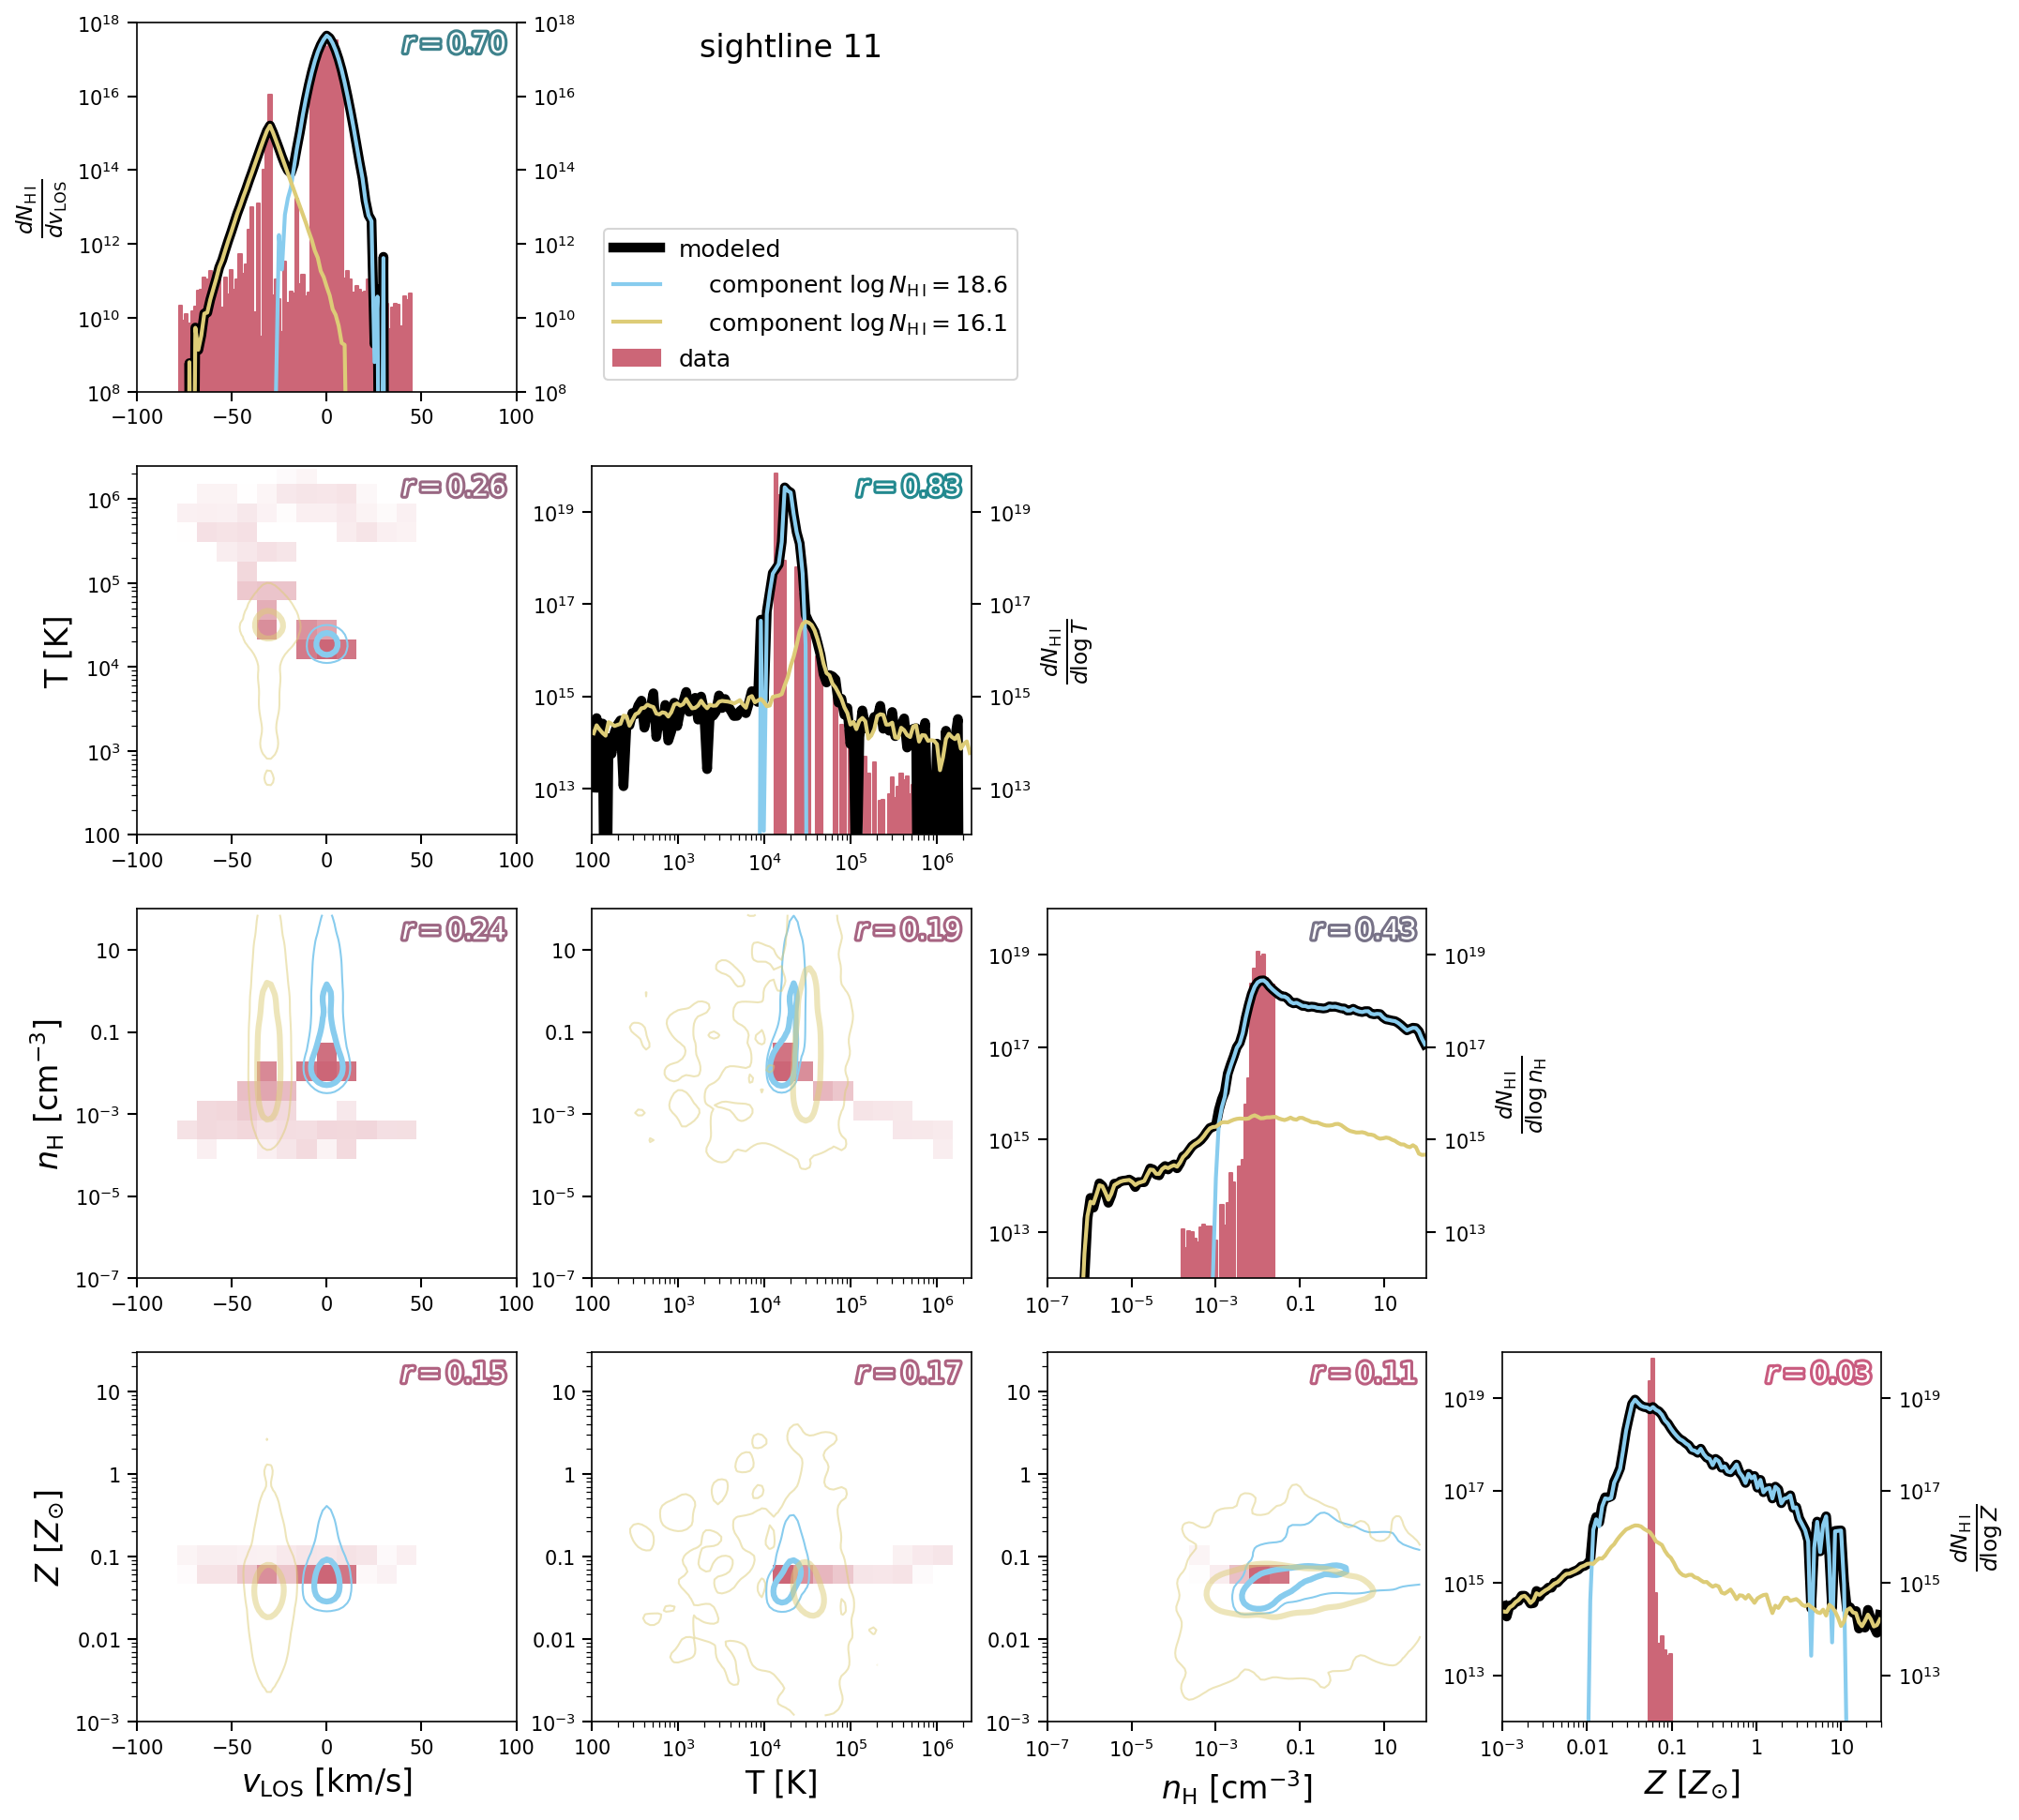
\includegraphics[width=\textwidth]{figures/sample2/sightline_0011.png}
    \label{f: sample2 11}
    \caption{Same as Fig.~\ref{f: sample2 03}, but for sightline 11.}
\end{figure*}

\begin{figure*}
    \centering
    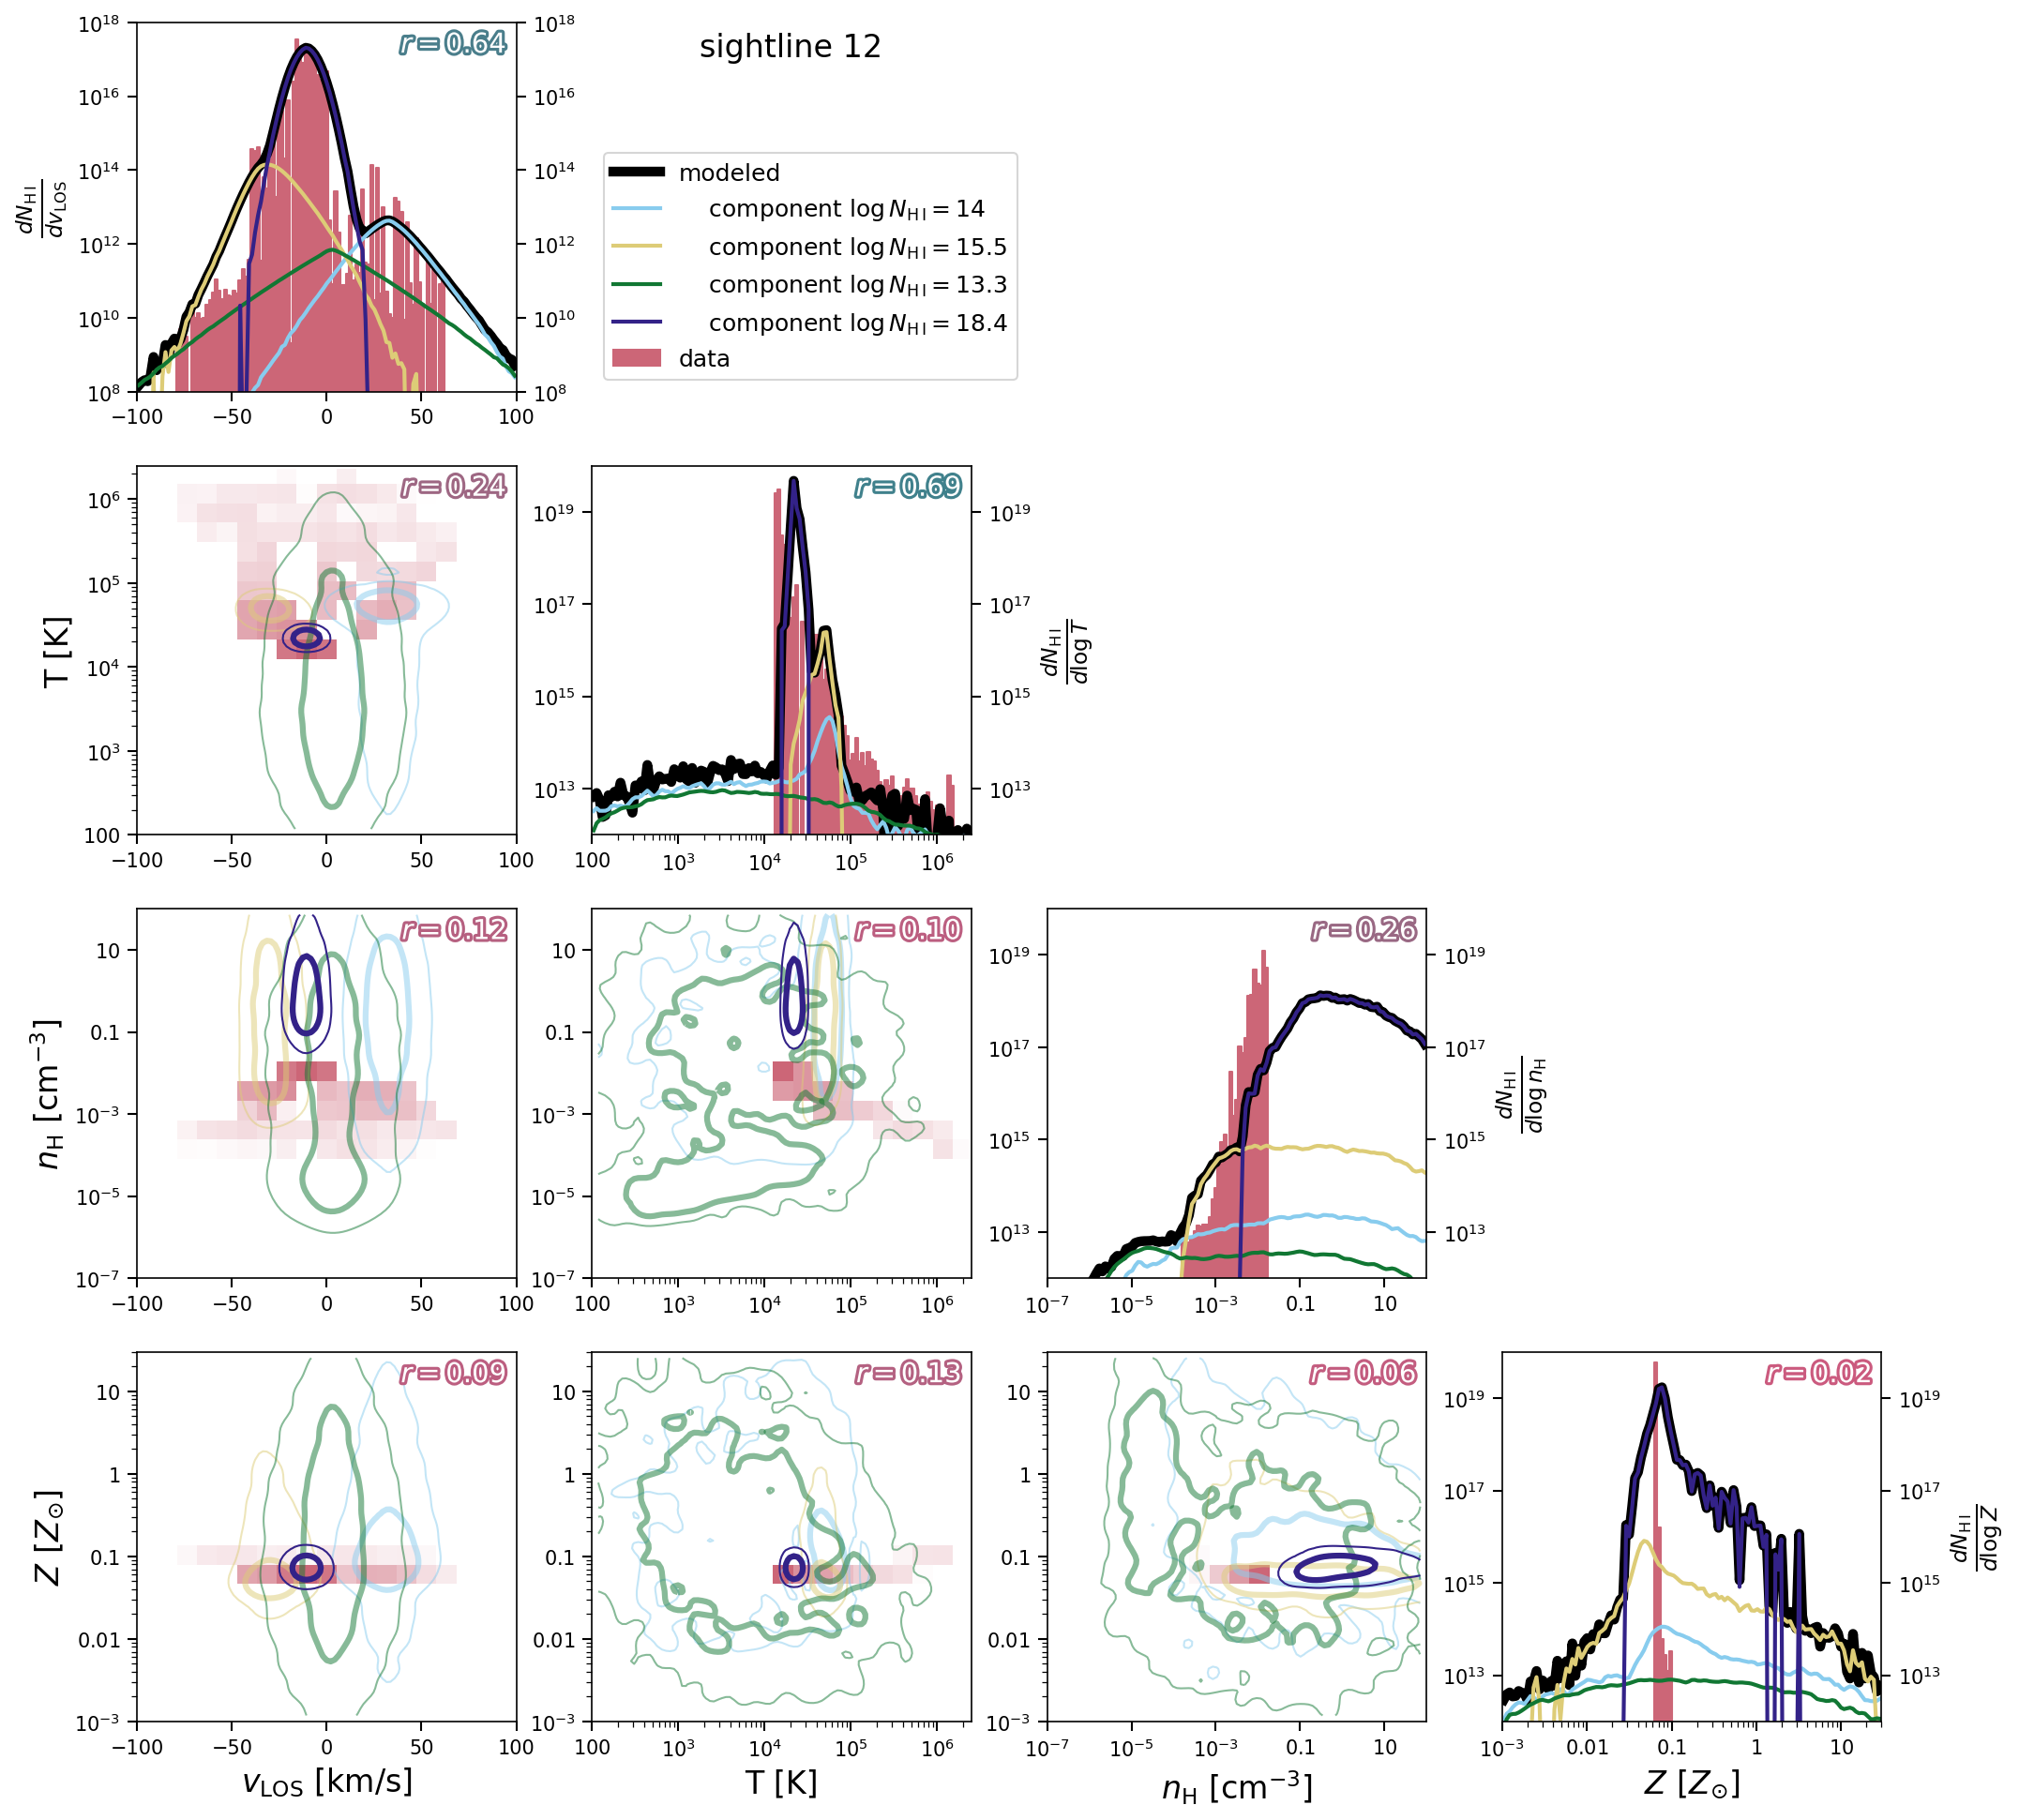
\includegraphics[width=\textwidth]{figures/sample2/sightline_0012.png}
    \label{f: sample2 12}
    \caption{Same as Fig.~\ref{f: sample2 03}, but for sightline 12.}
\end{figure*}

\begin{figure*}
    \centering
    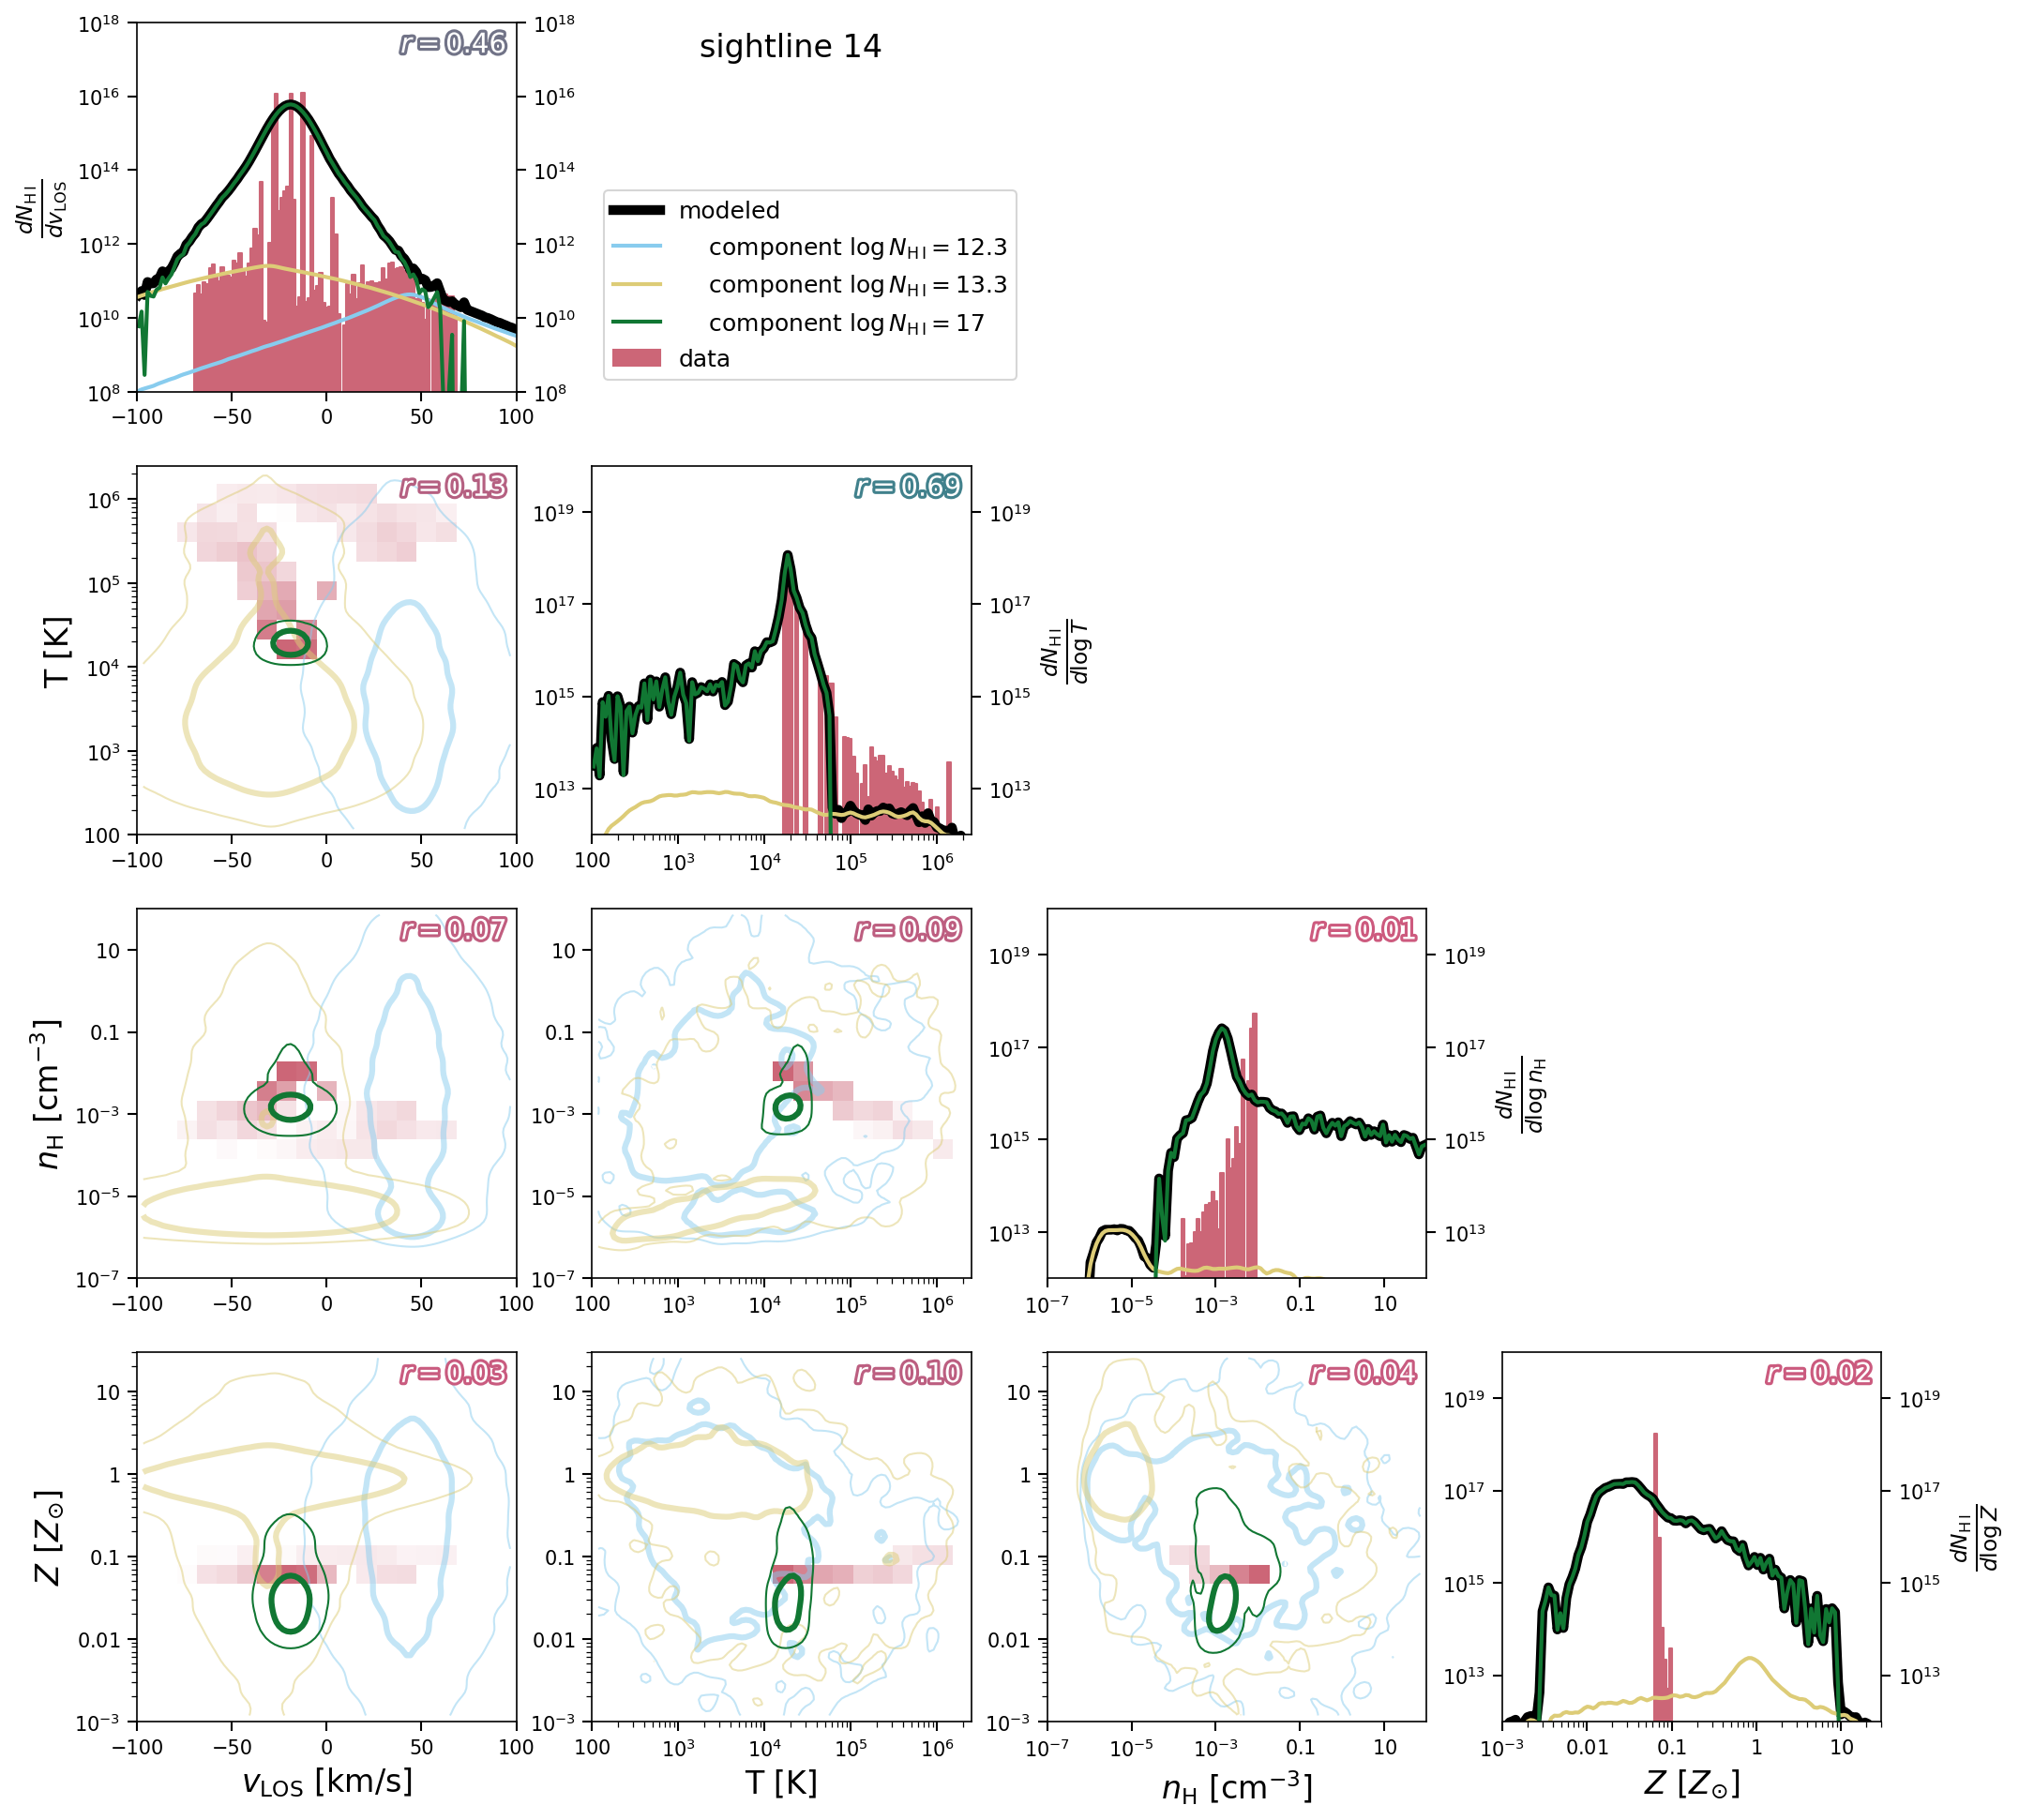
\includegraphics[width=\textwidth]{figures/sample2/sightline_0014.png}
    \label{f: sample2 14}
    \caption{Same as Fig.~\ref{f: sample2 03}, but for sightline 14.}
\end{figure*}

\begin{figure*}
    \centering
    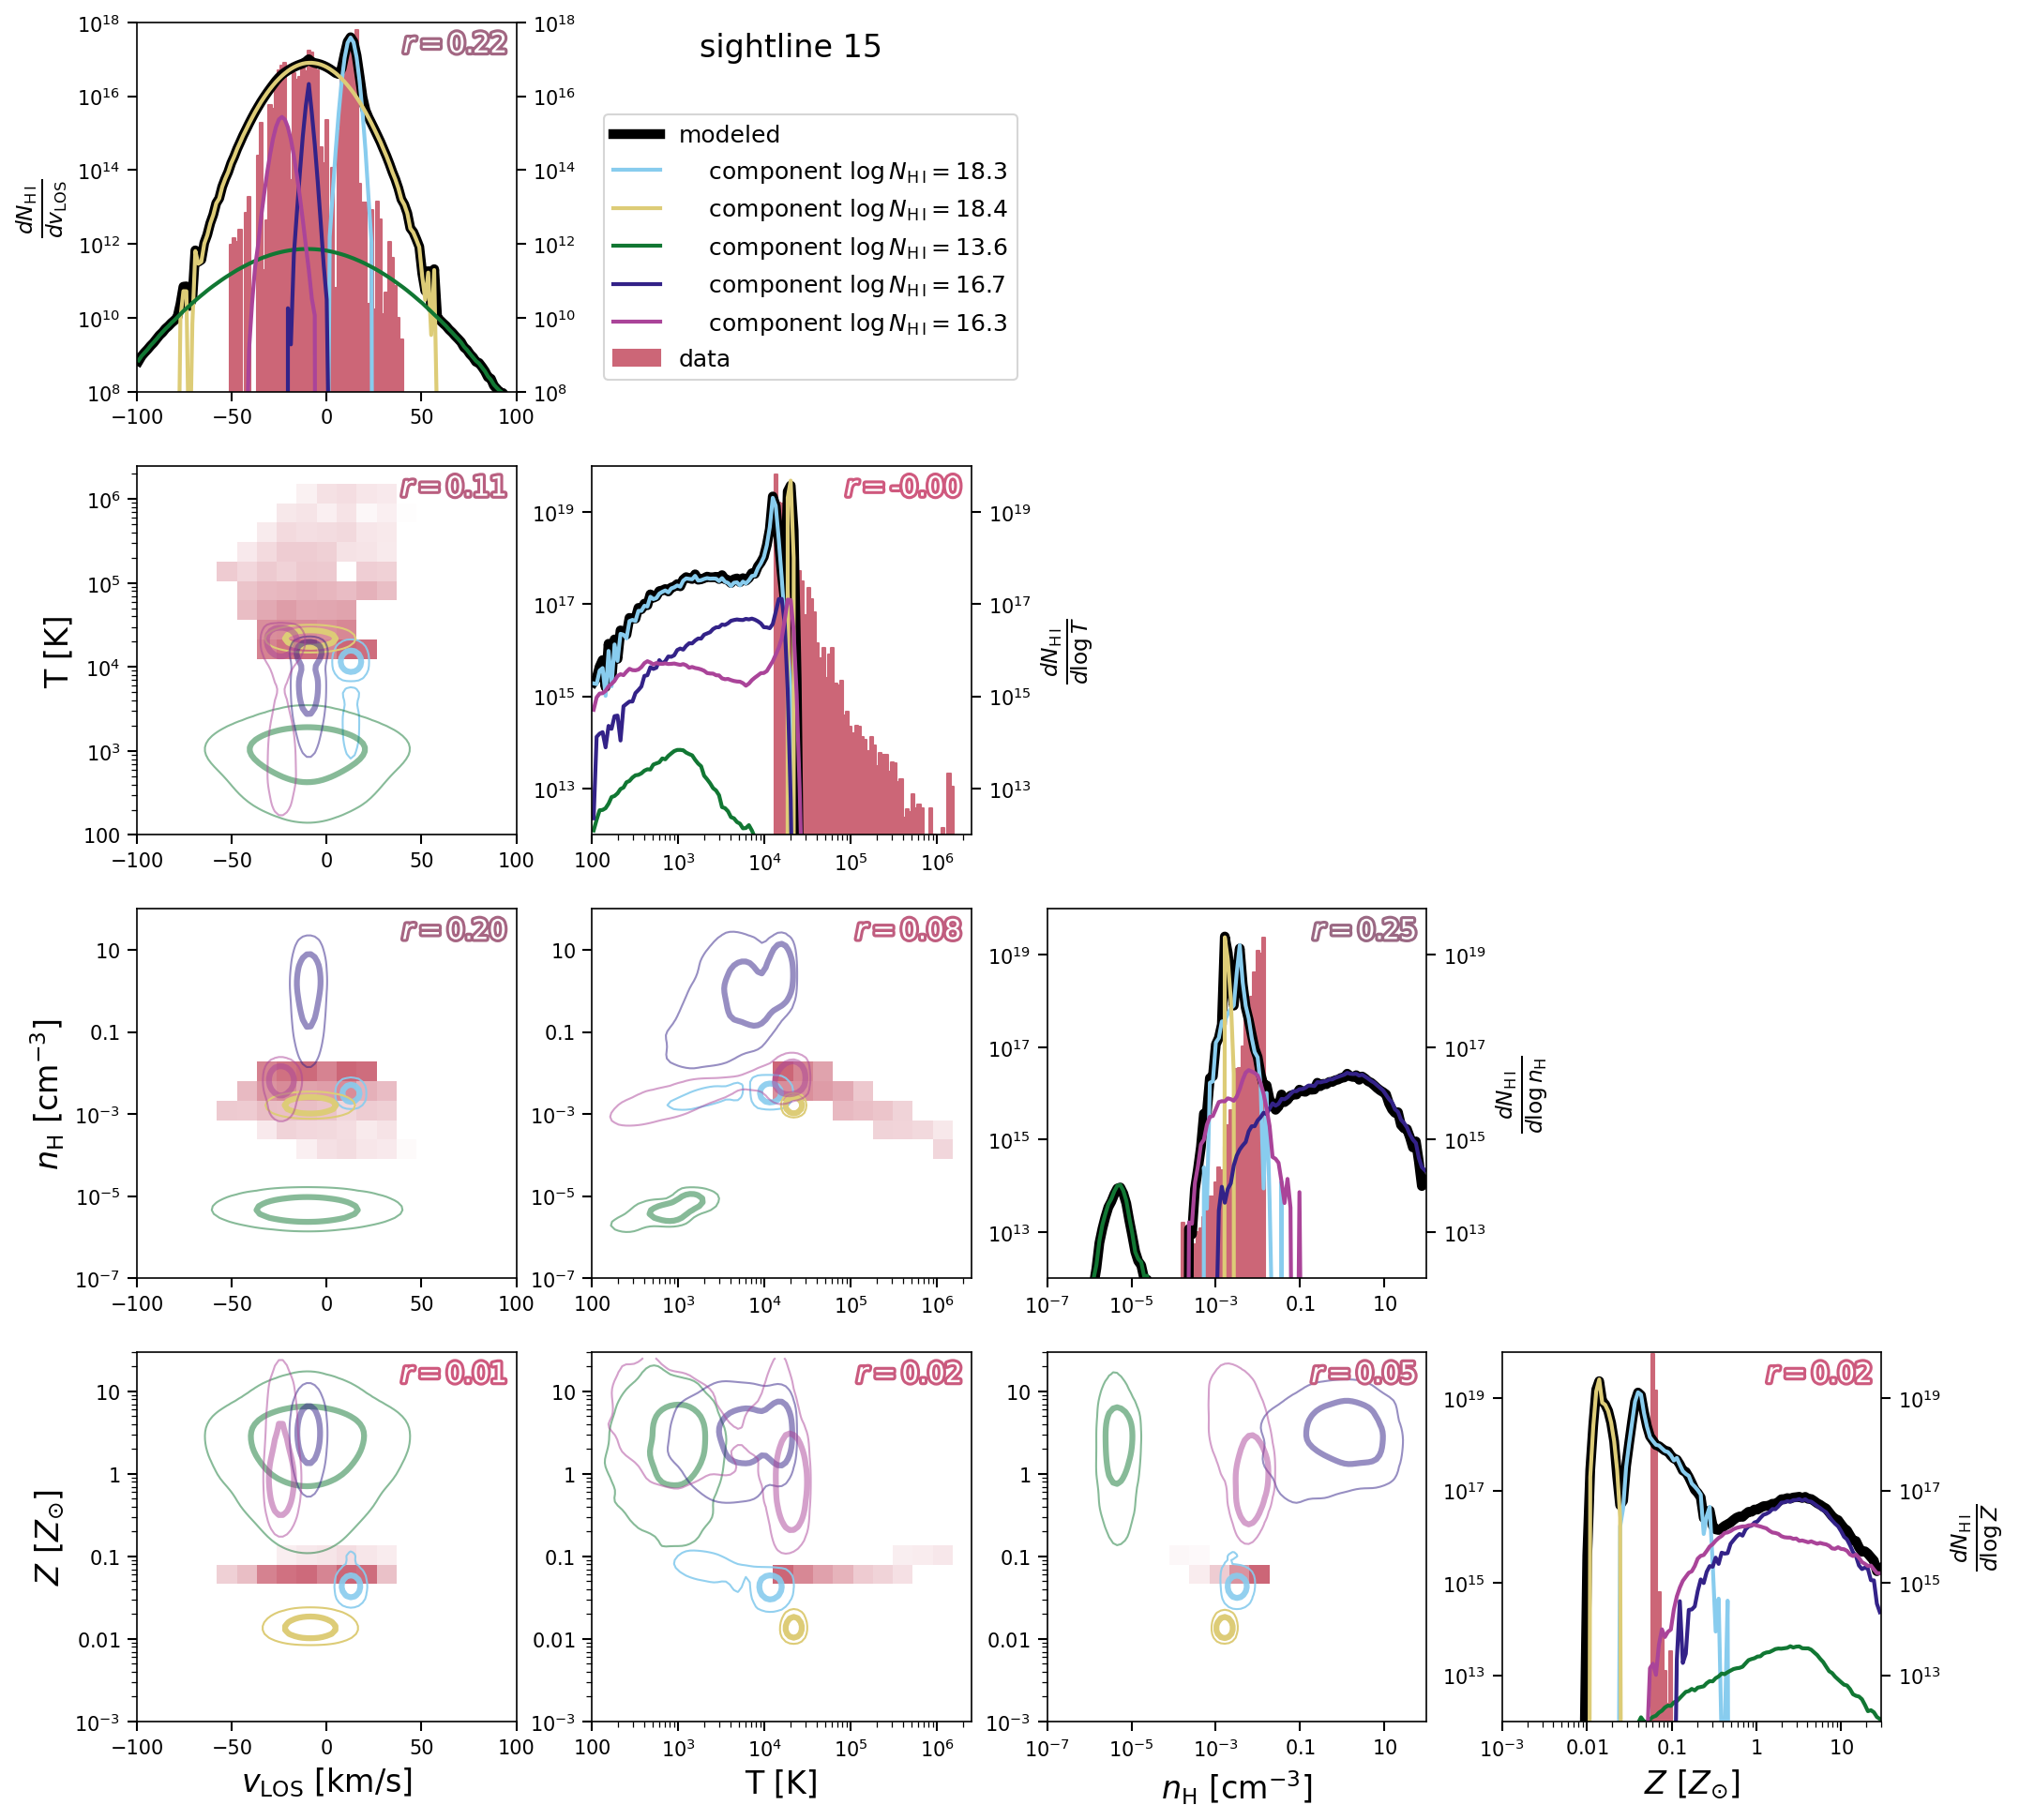
\includegraphics[width=\textwidth]{figures/sample2/sightline_0015.png}
    \label{f: sample2 15}
    \caption{Same as Fig.~\ref{f: sample2 03}, but for sightline 15.}
\end{figure*}

\begin{figure*}
    \centering
    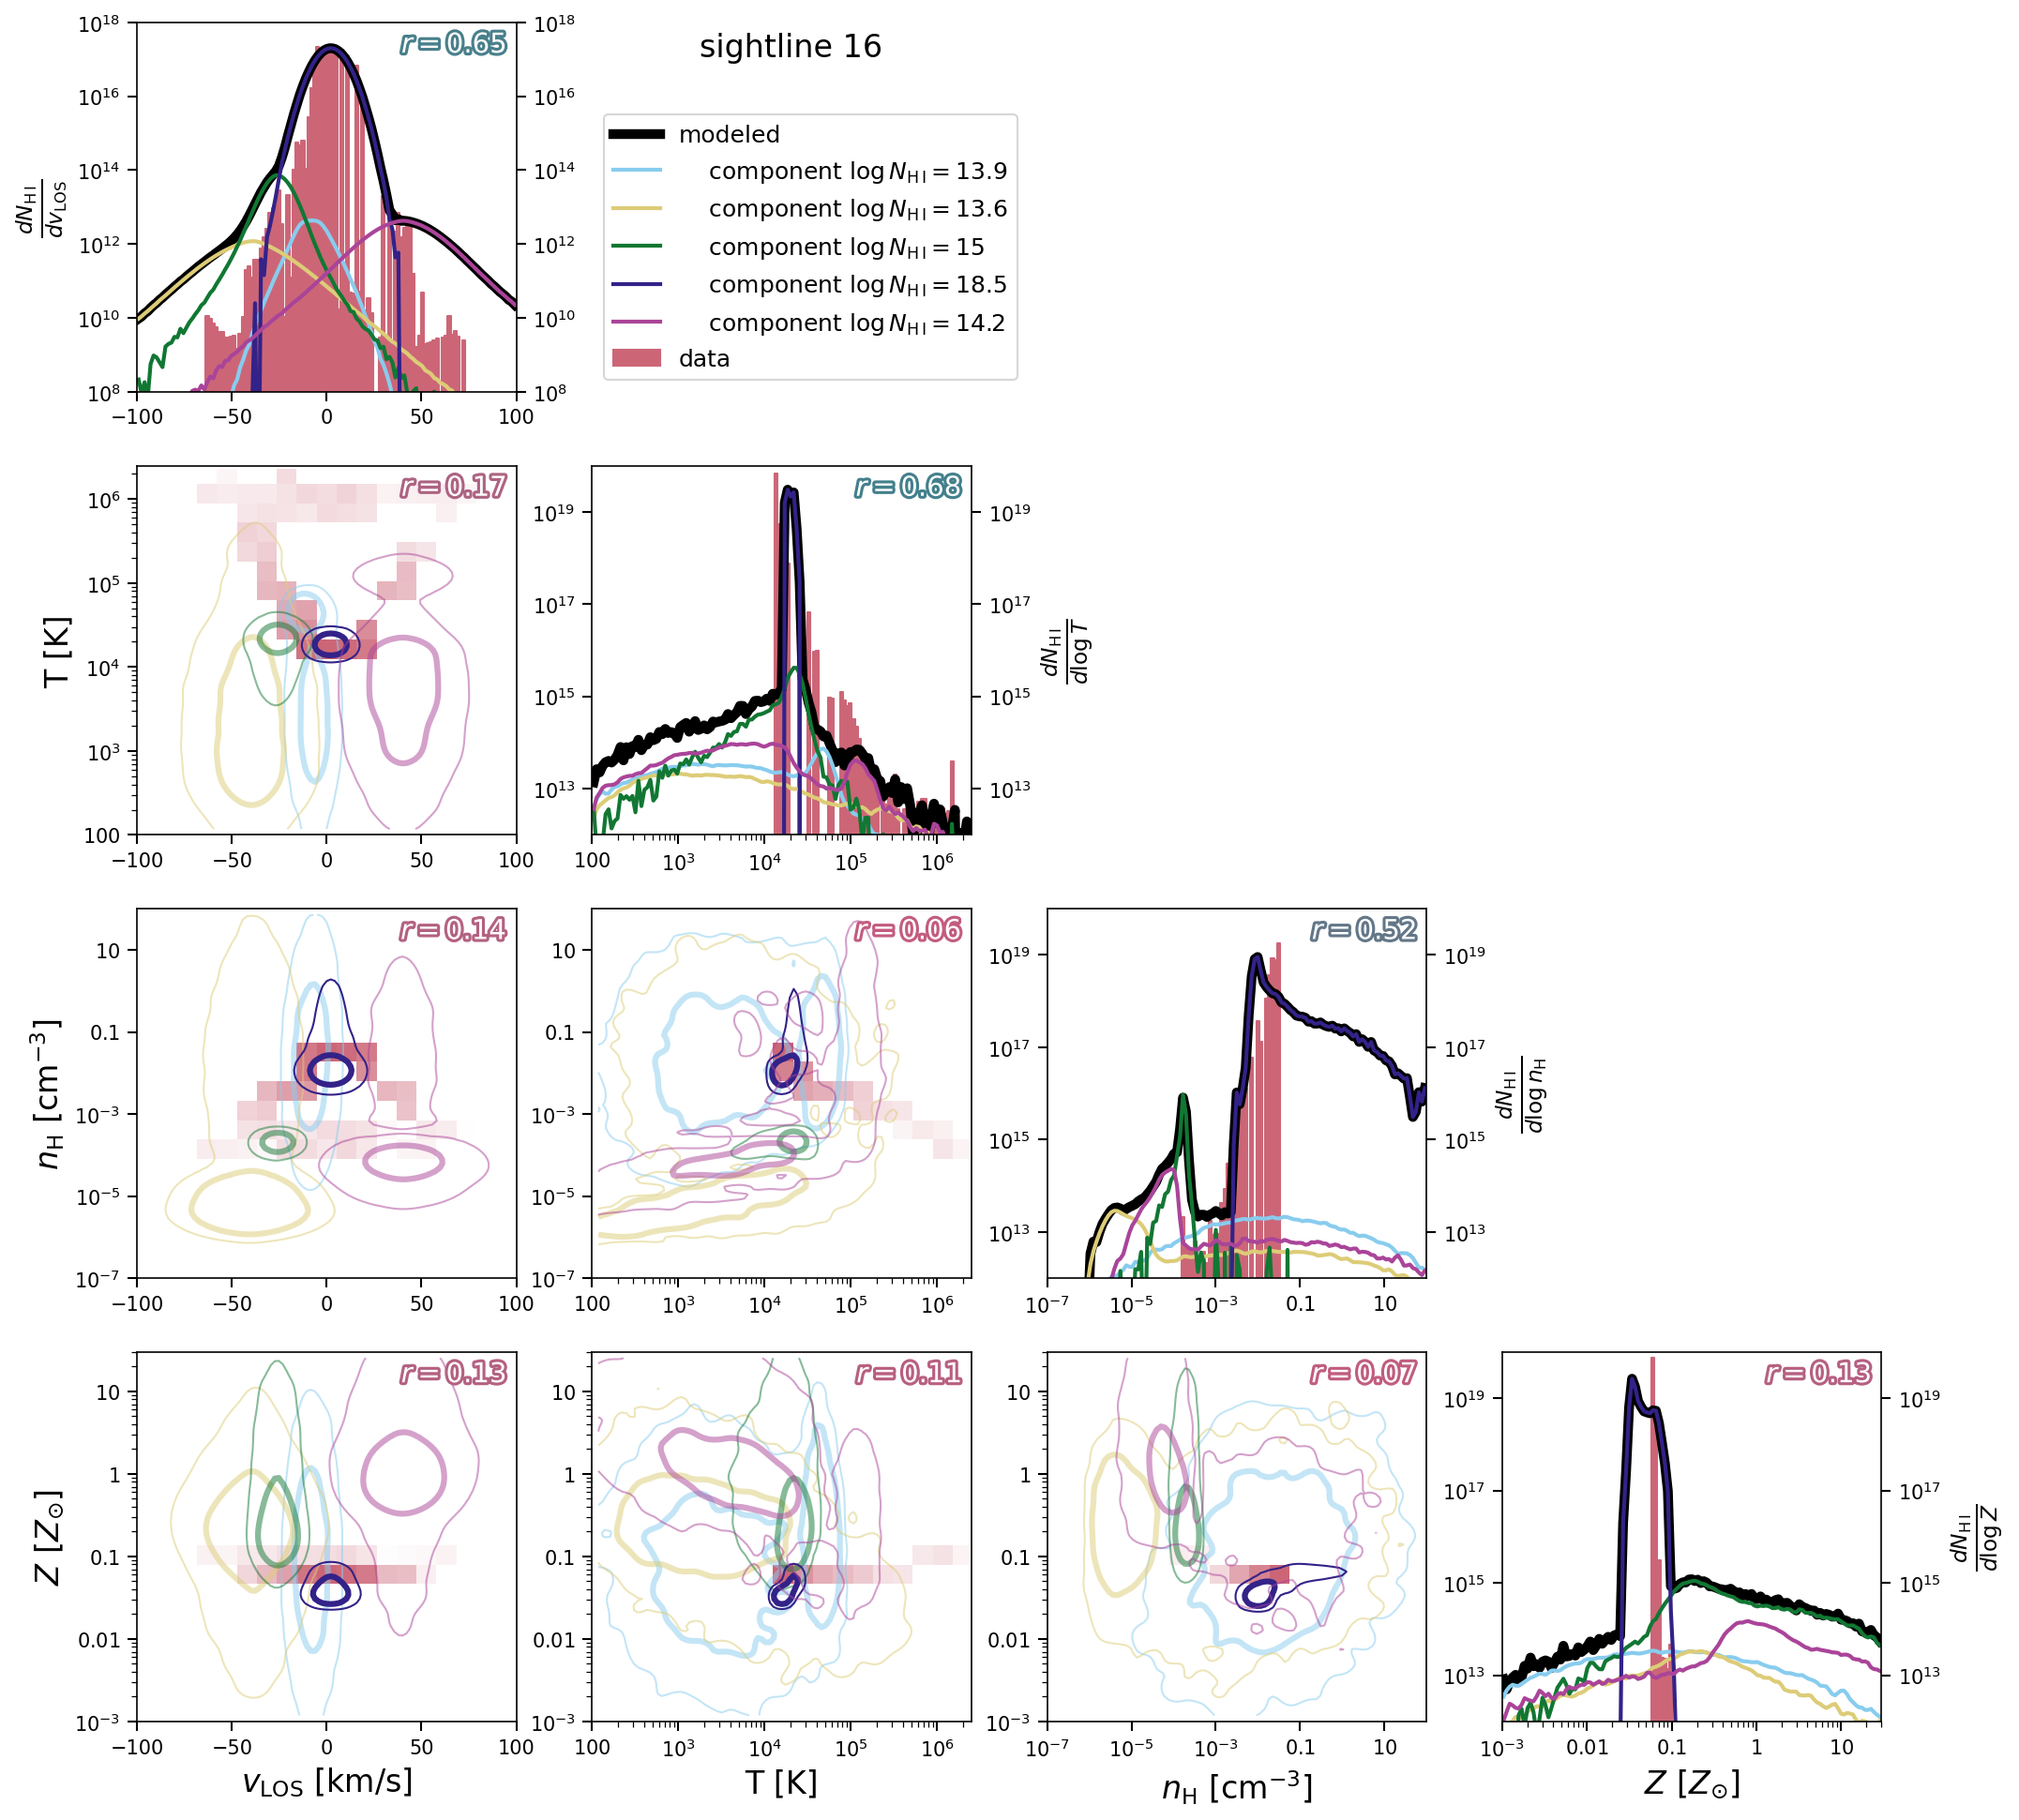
\includegraphics[width=\textwidth]{figures/sample2/sightline_0016.png}
    \label{f: sample2 16}
    \caption{Same as Fig.~\ref{f: sample2 03}, but for sightline 16.}
\end{figure*}

\begin{figure*}
    \centering
    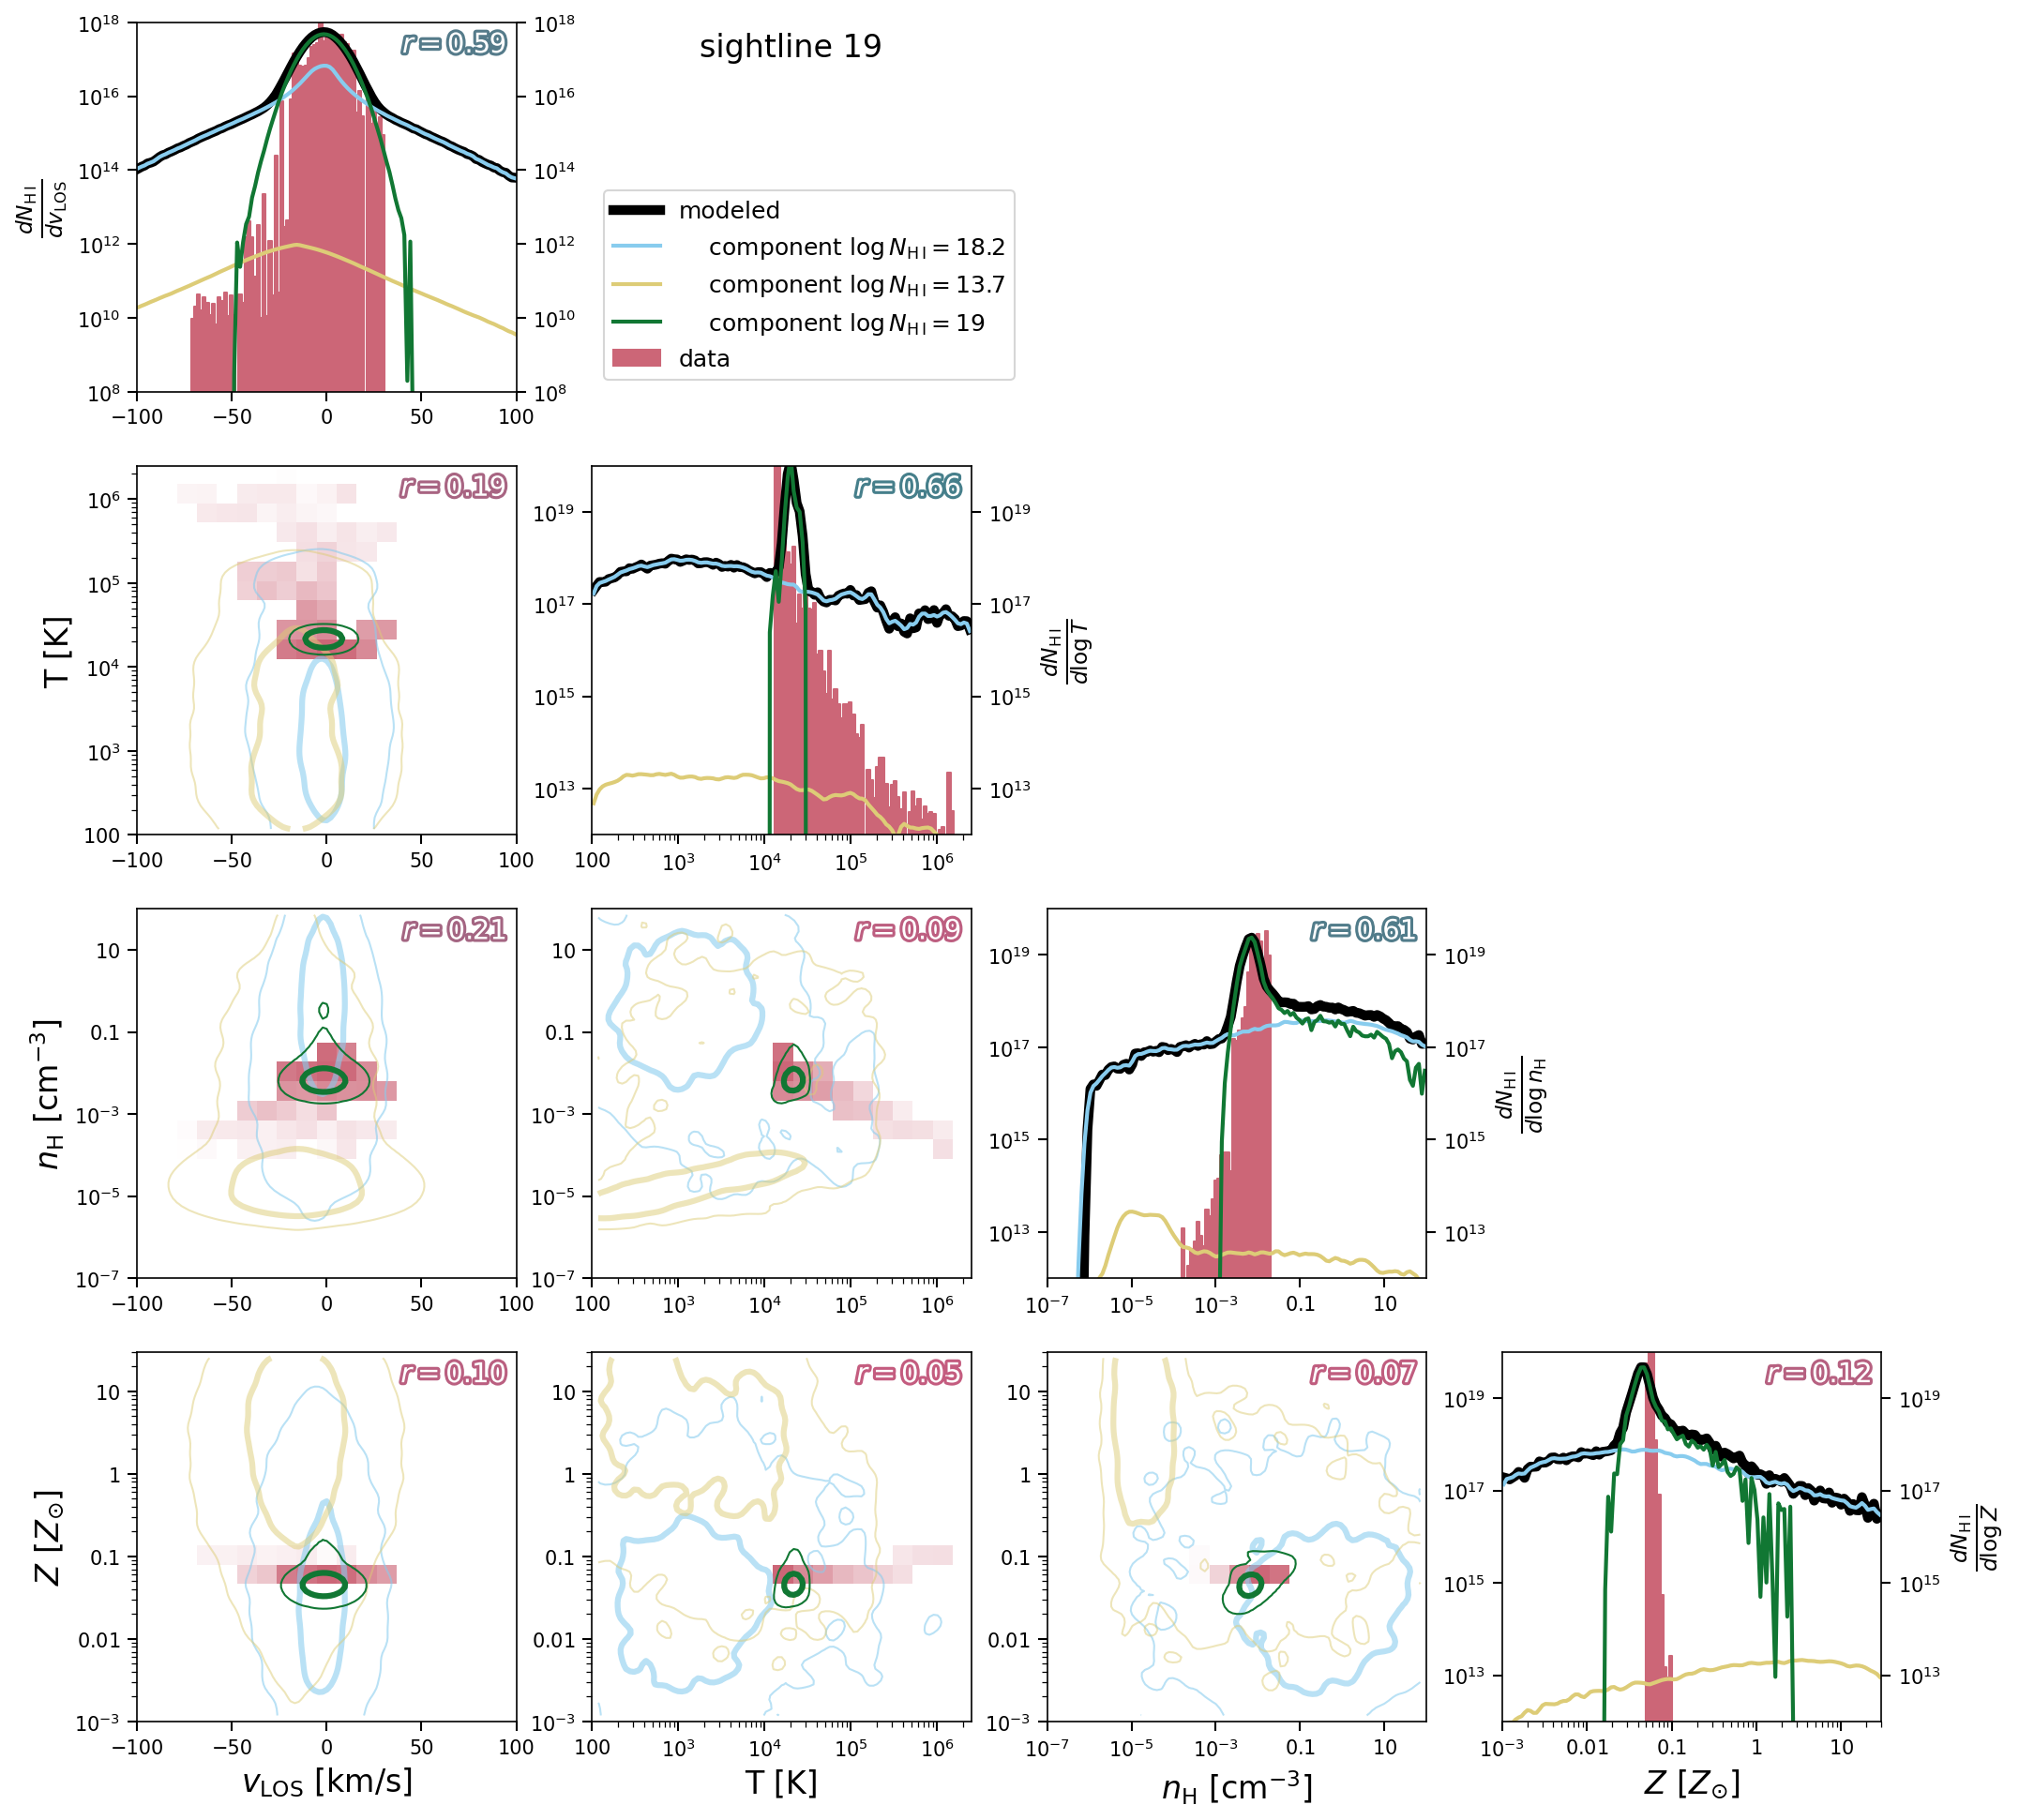
\includegraphics[width=\textwidth]{figures/sample2/sightline_0019.png}
    \label{f: sample2 19}
    \caption{Same as Fig.~\ref{f: sample2 03}, but for sightline 19.}
\end{figure*}

% Interpreting multi-component spectra
Absorbing gas with the same LOS-velocity is not necessarily co-spatial, but instead a single absorption component can correspond to multiple clouds of gas that are physically separated.
Analysis of mock absorption spectra from cosmological simulations shows that only $\sim 30-50\%$ of absorption components are composed of a single, contiguous cloud, and $\sim 50\%$ of multiple clouds contributing to a single component are separated by $\gtrsim 3-12$ kpc depending on ion~\citep[][]{Marra2022}.
Further, the amount of mass in common between velocity-aligned absorption from different ions varies widely, with $\sim 1/3$ of \ion{Si}{II} and \ion{C}{IV} absorbers sharing $>50\%$ of their mass~\citep[][]{Marra2022}.
These results are expected to be enhanced for higher-resolution simulations focused on individual filaments or clouds.

\note{
Follow-up analysis for this sample is currently ongoing.
The results section will be written at time of completion.
}

\atsameer{Commentary for this sample?}

\todo{Add comparison of mass-weighted average quantities.}

\todo{Discuss the high-density and also the low-temperature tails present often in modeling but not the actual data}

\section{Discussion}
\label{s: discussion}

\thoughts{Additional discussion topics.}

\subsection{What data is required for accurate modeling?}

\todo{What data is necessary in order to get the average properties right?}

\todo{What data is necessary to reproduce the simulated logspace distributions?}

\subsection{What level of agreement is necessary for modeling to be representative?}

\S\ref{s: results -- sample0} shows that reasonable agreement in ion column densities does not necessarily signal that the modeled properties are consistent with the actual properties.

\subsection{Implications for existing results}

% For analyses that infer a physical picture from individual sightlines
Some works argue that detailed information about the physical nature of the absorbing gas can be suggested, often with the aid of additional observations regarding the associated galaxy such as via IFU instruments (e.g. \citealt{Peroux2013}, who identify some of their systems as outflows; or \citealt{Peroux2017}, who exclude outflows).
Do our results throw any doubt into the mix about these models, or are they safe?

% For analyses that infer total masses or mass profiles
Some works aim to constrain total masses or mass profiles~\citep[e.g.][]{Zahedy2019a}.
Are these estimates affected?

\subsection{Modeling choices}

\subsubsection{Discrete components versus a distributions of cloud properties}

% Interpreting posteriors of single clouds as distributions.
Absorbers in reality are likely composed of infinitely many clouds with a distribution of properties.
One method of estimating this distribution may be the same method, or very similar, as used to estimate the PDF for a finite number of uniform clouds.
The argument is as follows.
When interpreting multiple components in an absorption system the classic interpretation is discrete clouds with uniform ($Z$, $n_{\rm H}$, $T$, $\NHI$), and uncertainty reflecting data noise.
However, we argue we can estimate $\frac{d\NHI}{dT}$ ( or $\frac{d\NHI}{dv_{\rm LOS}}$, etc.) using posteriors produced during observational modeling.
For simplicity and generality of discussion during the following we will be referring to $\frac{dM}{dx}$, where $M$ is an extrinsic mass quantity (e.g. $\NHI$) and $x$ is an intrinsic property (e.g. temperature).
Assume the total $\frac{dM}{dx}$ is well described by $q$ different distributions, i.e. $\frac{dM}{dx} = \sum_{i=1}^{q} \frac{dM_i}{dx}$.
If we had a way to estimate each individual $\frac{dM_i}{dx}$ we could therefore estimate the total $\frac{dM}{dx}$.
We note that $\frac{dM_i}{dx}$ is equivalently $\frac{dM_i}{dx} = M_i \frac{da}{dx}$, where $M_i$ is the total mass of component $i$ and $\frac{da}{dx}$ is defined as the fraction of mass with a given x, s.t. $\int dx \frac{da}{dx} = 1$.
Note that while $\frac{da}{dx}$ has similar properties as the posterior $f(x)$, we have not yet argued that $f(x)$ may be a good representation of it.
To estimate $\frac{da}{dx}$ I would argue we would want to use some method that estimates fraction of $M_i$ at a given $x$ based on
(a) the actual fraction of $M_i$ at x, and
(b) uncertainties in the estimation of $\frac{da}{dx}$.
This is similar to what the method of estimating $f(x)$ does.
Consider the limit of zero uncertainty but the absorption system having a distribution of properties instead of a single property.
We hypothesize that the method of estimating $f(x)$ would in such a case trace produce an $f(x)$ that traces the distribution.
We leave testing of this to future work \todo{Do we?}.
As such, we use $f(x)$ as an estimate for $dfrac{da}{dx}$. Therefore we have an estimate for $\frac{dM}{dx}$ using the estimated pdfs,
$\frac{dM}{dx} = \sum_{i=1}^{q} M_i f(x)$, and in turn $\frac{d\NHI}{dT} = \sum_{i=1}^{q} N_{\ion{H}{I},\,i} f(T)$.
\todo{There's at least one flaw in this argument.
When checking the fit Sameer uses the discrete properties of multiple clouds, not multiple distributions.
As such some of the individual clouds may "try" to balance missing data from the other clouds.}

\subsubsection{Absorption modeling ``by hand''}

There are a number of works that use a less-algorithmic, more people-driven approach to model sightlines~\citep[e.g.][]{Lacki2010}.
How does the modeling done here compare?
\atsameer{This is a question especially for you.}

\subsection{Comparison to similar analyses}

% Mock CGM analyses of robustness of modeling.
\cite{Liang2018} determined that a Bayesian method of modeling absorption lines was able to derive LOS mass-weighted average properties.
\cite{Marra2021} confirmed this finding using a blind study of spectra from cosmological simulations of a $z=1$ Milky Way-type galaxy and a $z=0$ dwarf galaxy.
\cite{Acharya2021} test the robustness of density and metallicity to changes in the UV background, and find that these quantities are uncertain by factors of $\approx 4-6.3$ and $\approx 1.6-3.2$ respectively.
\cite{Sameer2021} 

\subsection{Other questions}

1). The adopted priors for the modelers are quite large. So, portions of the parameter space that are not present in the simulation space could also be picked up during the modeling.
2). The highest resolution in the simulation is ~ 47 pc. Should there be a consideration of the size scales when modeling? For observational data, though, we don't have such a luxury of imposing constraints.
3). How does the cloud-in-cell interpolation affect the results, particularly volume-weighted density and mass-weighted temperature? Can't they be left variable from cell-to-cell instead of weighting in certain ways?

The inferred line of sight thickness with the modeling in some cases is $\ll$ sub-pc scale.
However, the simulation is only resolving clouds > 47 pc, so it could be a good idea if it is physically motivated to set an informed prior on the line of sight thickness of clouds

\section{Conclusions}
\label{s: conclusions}

The last numbered section should briefly summarise what has been done, and describe
the final conclusions which the authors draw from their work.

\section*{Acknowledgements}

This work exists thanks to the Halo21 KITP virtual conference, organized by Cameron Hummels, Ben Oppenheimer, Mark Voit, and Jess Werk.
This research was supported in part by the National Science Foundation under Grant No. NSF PHY-1748958.

%%%%%%%%%%%%%%%%%%%%%%%%%%%%%%%%%%%%%%%%%%%%%%%%%%
\section*{Data Availability}

 
The inclusion of a Data Availability Statement is a requirement for articles published in MNRAS. Data Availability Statements provide a standardised format for readers to understand the availability of data underlying the research results described in the article. The statement may refer to original data generated in the course of the study or to third-party data analysed in the article. The statement should describe and provide means of access, where possible, by linking to the data or providing the required accession numbers for the relevant databases or DOIs.




%%%%%%%%%%%%%%%%%%%% REFERENCES %%%%%%%%%%%%%%%%%%

% The best way to enter references is to use BibTeX:

\bibliographystyle{mnras}
\bibliography{references} % if your bibtex file is called example.bib

%%%%%%%%%%%%%%%%%%%%%%%%%%%%%%%%%%%%%%%%%%%%%%%%%%

%%%%%%%%%%%%%%%%% APPENDICES %%%%%%%%%%%%%%%%%%%%%

\appendix

\section{Some extra material}

If you want to present additional material which would interrupt the flow of the main paper,
it can be placed in an Appendix which appears after the list of references.

%%%%%%%%%%%%%%%%%%%%%%%%%%%%%%%%%%%%%%%%%%%%%%%%%%


% Don't change these lines
\bsp	% typesetting comment
\label{lastpage}
\end{document}

% End of mnras_template.tex
